\documentclass[a4paper,12pt]{book}
\usepackage{mathptmx}
\usepackage{hyperref}
\usepackage{cancel}
\usepackage{amsmath}
\usepackage{amssymb}
\usepackage{graphicx}
\usepackage{pgfplots}
\usepackage{tikz}
\usepackage{pgfplots}
\usepackage{xcolor}

\author{Gábor Hadházy and Tamás Hadházy}
\title{Mathematics}
\date{\today}

\begin{document}
\maketitle

\tableofcontents

% Chapter 1 - Algebra
\chapter{Algebra and Pre-calculus}
The first chapter is about algebra. It will cover the topics that was written by Gábor Hadházy and Tamás Hadházy. Algebra and Pre-calculus are the foundation of mathematics. It is important to understand the concepts of algebra and pre-calculus before moving on to more advanced topics.

\section{Essentials}
This section will cover the essentials in order to get started. 
\subsection{The set of Real numbers}
\begin{itemize}
    \item $\mathbb{N} = \{1, 2, 3, ...\}$ - - The set of natural numbers. 
    \item $\mathbb{Z} = \{..., -2, -1, 0, 1, 2, ...\}$ - The set of integers.
    \item $\mathbb{Q} = \{\frac{a}{b} | a, b \in \mathbb{Z}, b \neq 0\}$ - The set of rational numbers. 
    \item $\mathbb{I}$ - The set of Irrational Numbers(Real numbers that are not rational). 
    \item $\mathbb{R} = \mathbb{Q} \cup \mathbb{I}$
\end{itemize}


\subsection{The properties of Real numbers}
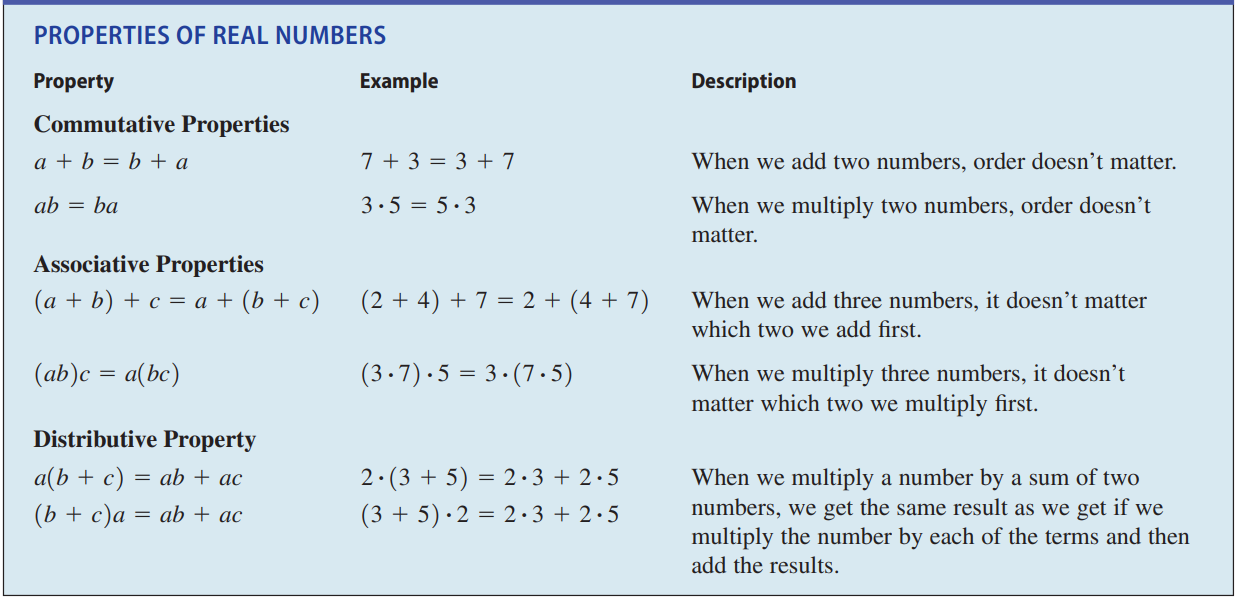
\includegraphics[width=1.1\textwidth]{algebra-pre-calculus/essentials/properties.png}

\subsection{Addition and Subtraction}
The number 0 is special for addition; it is called the additive identity because $a+0=a$ for any real number $a$. Every real number $a$ has a negative, $-a$, that satisfies $a+(-a)=0$. Subtraction is the operation that undoes addition; to subtract a number from another, we simply add the negative of that number. By definition
$$
a-b=a+(-b)
$$
To combine real numbers involving negatives, we use the following properties.
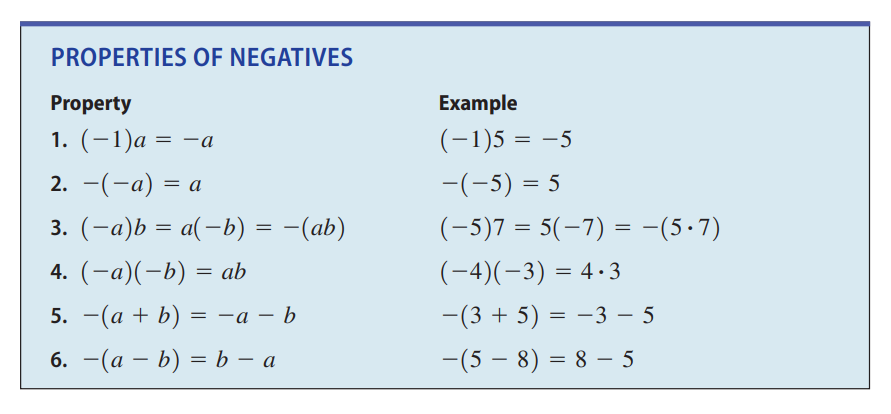
\includegraphics[width=1.1\textwidth]{algebra-pre-calculus/essentials/properties_addition_subtraction.png}

Property 6 states the intuitive fact that $a-b$ and $b-a$ are negatives of each other. \\
Property 5 is often used with more than two terms:
$$
    -(a+b+c)=-a-b-c
$$

\subsection{Multiplication and Division}
The number 1 is special for multiplication; it is called the \textbf{multiplicative identity} because $a \cdot 1=a$ for any real number $a$. Every nonzero real number $a$ has an inverse, $1 / a$, that satisfies $a \cdot(1 / a)=1$. Division is the operation that undoes multiplication; to divide by a number, we multiply by the inverse of that number. If $b \neq 0$, then, by definition,
$$
a \div b=a \cdot \frac{1}{b}
$$
We write $a \cdot(1 / b)$ as simply $a / b$. We refer to $a / b$ as the quotient of $a$ and $b$ or as the fraction $a$ over $b$; $a$ is the numerator and $b$ is the denominator (or divisor). To combine real numbers using the operation of division, we use the following properties. \\
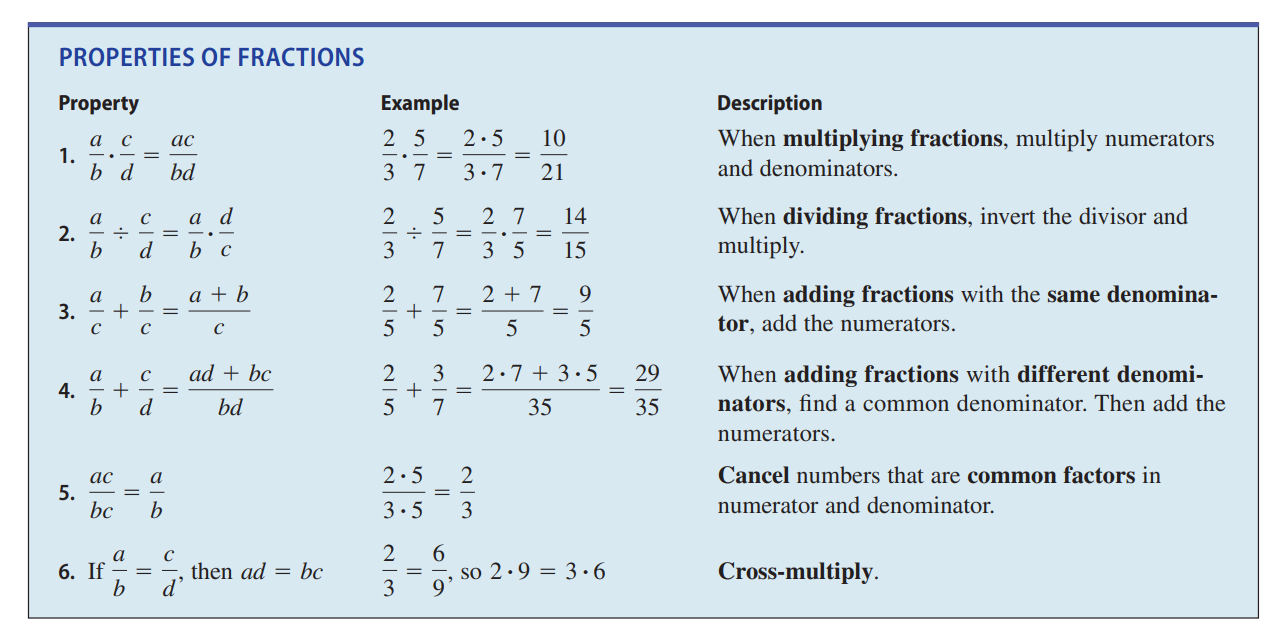
\includegraphics[width=1.1\textwidth]{algebra-pre-calculus/essentials/properties_multiplication_division.png}

When adding fractions with different denominators, we don’t usually use Property 4.
Instead we rewrite the fractions so that they have the smallest possible common denominator (often smaller than the product of the denominators), and then we use Property 3. This
denominator is the Least Common Denominator (LCD) described in the next example.

\subsection{Using the LCD to Add Fractions}

Evaluate: $\frac{5}{36}+\frac{7}{120}$
\textbf{Solution.} Factoring each denominator into prime factors gives
$$
36=2^2 \cdot 3^2 \quad \text { and } \quad 120=2^3 \cdot 3 \cdot 5
$$
We find the least common denominator (LCD) by forming the product of all the prime factors that occur in these factorizations, using the highest power of each prime factor. Thus the LCD is $2^3 \cdot 3^2 \cdot 5=360$. So
$$
\begin{aligned}
\frac{5}{36}+\frac{7}{120} & =\frac{5 \cdot 10}{36 \cdot 10}+\frac{7 \cdot 3}{120 \cdot 3} & \text { Use common denominator } \\
& =\frac{50}{360}+\frac{21}{360}=\frac{71}{360} & \begin{array}{l}
\text { Property } 3: \text { Adding fractions with the } \\
\text { same denominator }
\end{array}
\end{aligned}
$$

\subsection{Real line}

The real numbers can be represented by points on a line, as shown below. The
positive direction (toward the right) is indicated by an arrow. We choose an arbitrary
reference point O, called the origin, which corresponds to the real number 0. Given any
convenient unit of measurement, each positive number x is represented by the point on
the line a distance of x units to the right of the origin, and each negative number -x is
represented by the point x units to the left of the origin. The number associated with the
point P is called the coordinate of P, and the line is then called a coordinate line, or a
real number line, or simply a real line. Often we identify the point with its coordinate
and think of a number as being a point on the real line.

\begin{align*}
    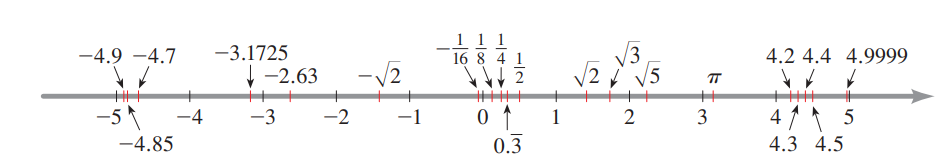
\includegraphics[width=1.1\textwidth]{algebra-pre-calculus/essentials/real-line.png}
\end{align*}

\section{Absolute Value and Distance}
The absolute value of a number $a$, denoted by $|a|$ , is the distance from $a$ to 0 on
the number line. Distance is always positive or zero, so we have
$|a|\geq0$ for every number $a$. Remembering that $-a$ is positive when $a$ is negative, we have the following definition.

\begin{equation*}
    |a| = \begin{cases}
        \;a  & \textnormal{if} \ a \geq 0 \\
        \;-a & \textnormal{if} \ a < 0
    \end{cases}
\end{equation*}

(a) $|3|=3$ \\
(b) $|-3|=-(-3)=3$ \\
(c) $|0|=0$ \\
(d) $|3-\pi|=-(3-\pi)=\pi-3 \quad($ since $3<\pi \quad \Rightarrow \quad 3-\pi<0)$

\subsection{Properties of Absolute Value}
\begin{enumerate}
    \item $|a| \geq 0$
    \item $|a|=|-a|$
    \item $|a b|=|a||b|$
    \item $\displaystyle \left|\frac{a}{b}\right|=\frac{|a|}{|b|}$
    \item $|a+b| \leq|a|+|b|$
\end{enumerate}

\subsection{Distance Between Points on the Real line}

What is the distance on the real line between the numbers -2 and 11? From
Figure 11 we see that the distance is 13. We arrive at this by finding either
$ |11-(-2)|=13$ or $|(-2)-11=13|$. From this observation we make the following definition. \\

If $a$ and $b$ are real numbers, then the \textbf{distance} between the points $a$ and $b$ on the real line is: \\
$$ d(a,b)=|a-b| $$

From the Property 6 of negatives it follows that
$$ |b-a| = |a-b|$$
$$ |3-7| = |7-3| = 4 $$

This confirms that, as we would expect, the distance from a to b is the same as the
distance from b to a.

\textbf{Example.} The distance between then numbers -8 and 2 is $d(-8,2)=|-8-2|=|-10|=10$.

\subsubsection*{Exercises}
For Exercises please download the book from here(\url{https://faculty.ksu.edu.sa/sites/default/files/precalculus-mathematics_for_calculus-j._stewart_l._redlin_and_s._watson-cengage_learning_7th_edition_2015.pdf}) and you can go to the 37th page for exercises.  % Section 1 - Essentials
\section{Exponentiation}
When starting out with Exponentiation it is important first to understand the different parts of an exponential expression, so let's consider:
$$b^x = \underbrace{b \cdot b \cdot ... \cdot b}_{x \ times}$$
\begin{itemize}
  \item $b$ is the \textbf{base}.
  \item $x$ is the \textbf{exponent}.
\end{itemize}

As a reminder $ x^0 = 1 $

Let's discuss the different rules of Exponentiation:
\subsection{Product Rule}
To find the product of two exponential expression with the same base, add the exponents. 
$$ x^{n} \cdot x^{m} = x^{n+m} $$

\subsection{Quotient Rule}
When two exponential expressions with the same base are divided,  to find their quotient subtract their exponents. 
$$ \frac{x^n}{x^m} = x^{n-m} $$

\subsection{Power Rule}
When you raise an power to a power in an exponential expression to get the product, multiply the exponents
$$ (x^{n})^{m} = x^{n \cdot m} $$ 
$$ OR $$
$$ (x^{n})^{m} = \underbrace{x^n \cdot ... \cdot x^n}_{m \ times} $$
Here it is proven that the power rule is simply just the product rule.

\subsection{Negative Exponents}
When dealing with negative exponents this equation will apply: 
$$ x^{-n} = \frac{1}{x^n} $$

Since, 
$$ \frac{1}{x} = \frac{x^0}{x^1} = x^{0-1} = x^{-1} $$
It is important to note that this is just only one way of proving this, there are a couple more. 

\subsection{Fractional Exponents}
$$ \large x^{\frac{1}{n}} = \sqrt[n]{x} $$
The proof of this can be found in the next section \hyperref[sec:radicals]{Radicals(click to redirect)}.

\subsection{Additional rules}
Distribute an exponent over a product: $(x \ y)^{n} = x^{n} \ y^{n}$ \\
Distribute an exponent over a quotient: $  (\frac{a}{b})^{n} = \frac{a^{n}}{b^{n}}$

\begin{align*}
  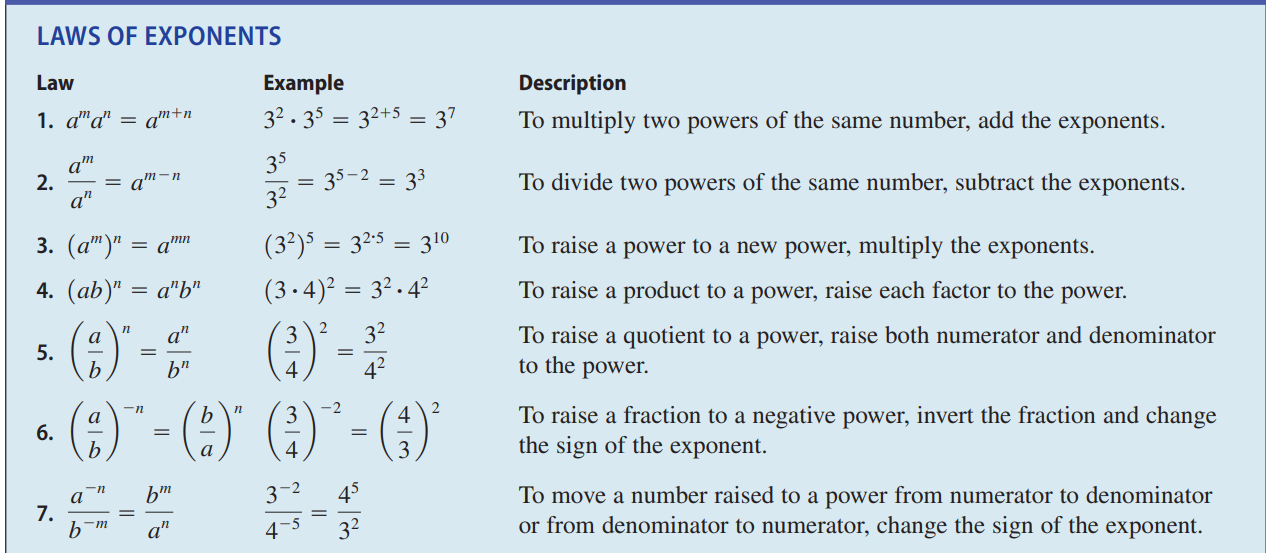
\includegraphics[width=1.2\textwidth]{algebra-pre-calculus/exponentiation/laws-of-exponents.png}
\end{align*}

\newpage % Section 2 - Exponentiation
\label{sec:radicals}
\section{Radicals}
$$ \large \sqrt[n]{x} $$
\begin{itemize}
  \item $x$ is the \textbf{radicand}.
  \item $n$ is the \textbf{index}(nth root).
  \item $\large \sqrt[n]{x}$ expression is the \textbf{radical}
\end{itemize}

As promised let's look at the fractional exponent equation. If $n$ is a positive integer that is greater than $1$ and a is a real number then,
$$ \sqrt[n]{a} = a^{\frac{1}{n}} $$

We are often referring the left side of the equation as the \textbf{radical form} and the right side of the equation as the \textbf{exponent form}

\subsubsection{Proof}
In order to prove this equation we can establish first this: 
$$ (a^{\frac{1}{n}})^{n} = a^{n \cdot \frac{1}{n}} = a^{\frac{n}{n}} = a $$
Let's take an example to avoid confusion: 
$$ (9^{\frac{1}{2}})^2 = 9^{\frac{1}{2} \cdot2} = 9^{\frac{2}{2}} = 9 $$

To put this into words $ 9^{\frac{1}{2}} $ is the number that when squared will return back $ 9 $. In other words this is exactly what it meant by the root(in this case square root) which will return back the number that when squared it will be 9. Therefore: 
$$ 9^{\frac{1}{2}} =  \sqrt[2]{9} = 3 $$

Since,
$$ (3)^2 = 9 = (9^{\frac{1}{2}})^2 $$

Therefore the equation has been proven: 
$$ \sqrt[n]{a} = a^{\frac{1}{n}} $$

It is very important to note a misconception here. The index is required in these radical expressions to make sure that we correctly evaluate the radical. There is one exception to this rule and that is square root.
$$ \sqrt[2]{a} = \sqrt[]{a} $$
In every other cases we \textbf{must} define the index, because otherwise it will be considered as a square root, Whenever working with square roots the index can be omitted.

\subsubsection{General rational exponent}
Since, $ a^{\frac{1}{n}} = \sqrt[n]{a} $.
Let's establish the general rational exponent in terms of radicals as follows. 
$$ a^{\frac{m}{n}} = (a^{\frac{1}{n}}) ^{m} = (\sqrt[n]{a})^m $$
$$ OR $$
$$ a^{\frac{m}{n}} = (a^m) ^{\frac{1}{n}} = \sqrt[n]{a^m} $$

Since being aware of the \textbf{Associative Property of Multiplication}, the order of the multiplication can be changed. 

Therefore, 
$$ a^{\frac{m}{n}} = \sqrt[n]{a^m} $$

\subsection{Properties of radicals}
\begin{itemize}
  \item $\sqrt[n]{a^n} = a$ \ This is simply true because when trying to find the $n$th root of a number and  also raising the number to that power then that's simply will be equal to the number.  \\
Consider this as an example,
$$ \sqrt[]{9^2} = \sqrt[]{81} = 9$$
   \item $ \sqrt[n]{ab} = \sqrt[n]{a} \sqrt[n]{b} $ \\
   To prove this consider this, \\
    1. Start with the left-hand side (LHS) of the equation,
    $ \sqrt[n]{ab} $ Using the definition of the nth root:
    $ \sqrt[n]{ab} = (ab)^{\frac{1}{n}} $ \\
    2. Next apply the product rule of exponents, which states that $ a^m \cdot a^n = a^{m+n} $ Therefore, $ (ab)^{\frac{1}{n}} = a^{\frac{1}{n}} \cdot b^{\frac{1}{n}} $ \\ 
    3. Now, rewrite the exponents as radicals:
    $ a^{\frac{1}{n}} $ is equivalent to $ \sqrt[n]{a} $ and $ b^{\frac{1}{n}} $ is equivalent to $ \sqrt[n]{b} $ \\
    4. So, we have: $ a^{\frac{1}{n}} \cdot b^{\frac{1}{n}} = \sqrt[n]{a} \cdot \sqrt[n]{b} $ \\
    5. Finally this proves that: $ \sqrt[n]{ab} = \sqrt[n]{a} \cdot \sqrt[n]{b} $
    \item $ \large \sqrt[n]{\frac{a}{b}} = \frac{\sqrt[n]{a}}{\sqrt[n]{b}} $ To prove this consider this, \\
    1. As previously Start with the left-hand side (LHS) of the equation: $ \sqrt[n]{\frac{a}{b}} $ \\
    2. Now using the definition of the nth root: $ \sqrt[n]{\frac{a}{b}} = \left(\frac{a}{b}\right)^{\frac{1}{n}} $ \\
    3. Apply the power rule of the exponents which states that: \\ $ (a^m)^{\frac{1}{n}} = a^{m \cdot \frac{1}{n}} = a^{\frac{m}{n}}$, Therefore when we are dealing with a fraction as the base it is the same when dealing with numbers that are not fractions: 
$$ \left(\frac{a}{b}\right)^{\frac{1}{n}} = \frac{a^{\frac{1}{n}}}{b^{\frac{1}{n}}} $$ Since, \\
$$ (\frac{a}{b})^c = \frac{a^c}{b^c} $$ \\
With an example: $ (\frac{a}{b})^2 = \frac{a}{b} \cdot \frac{a}{b} = \frac{a^2}{b^2} $ \\
	4. Now rewrite the exponents as radicals: $ a^{\frac{1}{n}} $ is equivalent to $ \sqrt[n]{a} $ and  $b^{\frac{1}{n}}$ is equivalent to $ \sqrt[n]{b} $ \\
	5. So, we have: 
	$$ \frac{a^{\frac{1}{n}}}{b^{\frac{1}{n}}} = \frac{\sqrt[n]{a}}{\sqrt[n]{b}} $$ \\
	6. Finally, this proves that: 
	$$ \sqrt[n]{\frac{a}{b}} = \frac{\sqrt[n]{a}}{\sqrt[n]{b}} $$ \\
	\\
	
	\item Also note that while we can “break up” products and quotients under a radical we can’t do the same thing for sums or differences. In other words,
	$$ \sqrt[n]{a+b} \neq \sqrt[n]{a}+ \sqrt[n]{b}  $$ 
	$$ AND $$
	$$ \sqrt[n]{a-b} \neq \sqrt[n]{a}- \sqrt[n]{b} $$ \\
These can simply be proven by examples, 
$$ 5 = \sqrt25 = \sqrt{9+16} \neq \sqrt9 + \sqrt16 = 3+4 = 7 $$

\end{itemize} % Section 3 - Radicals
\section{Algebraic Expressions}
A \textbf{variable} is a letter that can represent any number from a given set of numbers. If we
start with variables, such as $x$, $y$, and $z$, and some real numbers and combine them using
addition, subtraction, multiplication, division, powers, and roots, we obtain an \textbf{algebraic expression}. Here are some examples:

$$ 
    2x^2-3x+4 \quad \sqrt{x}+10 \quad \frac{y-2z}{y^2+4}
$$

A \textbf{monomial} is an expression of the form $ax^k$
, where a is a real number and k is a
nonnegative integer. A \textbf{binomial} is a sum of two monomials and a \textbf{trinomial} is a sum
of three monomials. In general, a sum of monomials is called a \textbf{polynomial}. For example, the first expression listed above is a polynomial, but the other two are not.

\begin{align*}
    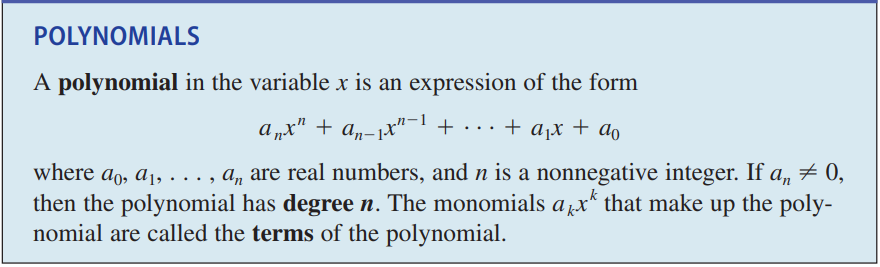
\includegraphics[width=1.1\textwidth]{algebra-pre-calculus/algebraic-expressions/polynomial definition.png}
\end{align*} \break

Note that the degree of a polynomial is the highest power of the variable that appears
in the polynomial.


\begin{align*}
    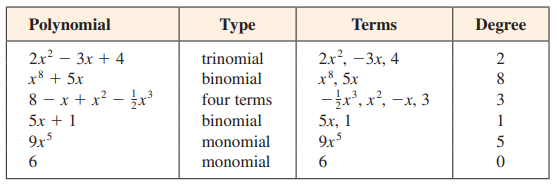
\includegraphics[width=1.1\textwidth]{algebra-pre-calculus/algebraic-expressions/algebraic-expression-spreadsheet.png}
\end{align*} \break

We add and subtract polynomials using the properties of real numbers that were discussed earlier. The idea is to combine like terms (that is, terms with the same
variables raised to the same powers) using the Distributive Property. For instance,

$$ 
    5x^7+3x^7-2x^7 = (5+3-2)x^7 = 6x^7
$$

But we already know this. 

To find the product of polynomials or other algebraic expressions, we need to use the
Distributive Property repeatedly. In particular, using it three times on the product of two
binomials, we get

$$ 
    (a+b)(c+d) = a(c+d)+b(c+d) = ac+ad+bc+bd
$$

\subsection{Special Product Formulas}
Certain types of products occur so frequently that you should memorize them. You can
verify the following formulas by performing the multiplications.

\begin{align*}
    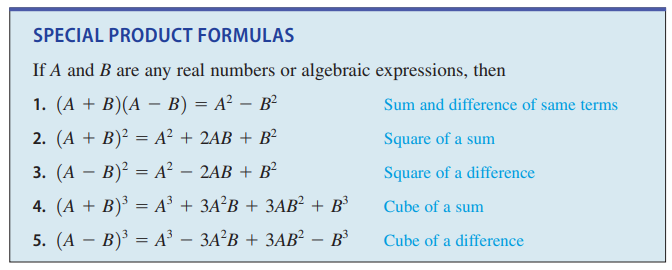
\includegraphics[width=1.1\textwidth]{algebra-pre-calculus/algebraic-expressions/special_product_formulas.png}
\end{align*} \break

\subsection{Factoring Common Factors}
We use the Distributive Property to expand algebraic expressions. We sometimes need
to reverse this process (again using the Distributive Property) by factoring an expression as a product of simpler ones.
For example,
\begin{align*}
    &A. \quad 15 + 25x = 5(3 + 5x) \\
    &B. \quad x^2y + y^2x^3 = x^2y(1 + xy) \\
\end{align*}
You can always check whether you have factored correctly by expanding the brackets.

\subsection{Factoring quadratics}
A quadratic is an expression with a squared term, then just a term with a variable, then a constant. 
\\ Like this: $ax^2 + bx + c$ 
More about solving quadratic equations and quadratic equations in general can be found in the next section \hyperref[sec:quadratic-equations]{Quadratic Equations(click to redirect)}.


We are looking for two numbers that multiply you get $c$ and when you add them you get $b$.
The reason why: 
$$ (x + m)(x + n) = \\ x^2 + mx + nx + mn = x^2 + \underbrace{(m + n)}_b x + \underbrace{(mn)}_c $$

$m$ and $n$ are the two numbers we are looking for. As you can see $m + n = b$ and $mn = c$. \\

\textbf{Example}. Factor $x^2 - 6x + 8$ \\
We are looking for two numbers that multiply you get $8$ and when you add them you get $-6$. \\
The two numbers are $-2$ and $-4$ because $-2 \cdot -4 = 8$ and $-2 + -4 = -6$. \\
Therefore, 
\begin{align*}
    x^2 - 6x + 8 &= (x - 2)(x - 4) \\
\end{align*}

\textbf{Example}. Factor $10x^2 + 11x - 6$ \\
\begin{itemize}
    \item Step 1. Multiply the leading coefficient (10) and the constant term (-6) to get -60. \\
    \textbf{Why?} The main goal in factoring a quadratic equation is to express it as the product of two binomials(like (2x+4)(4x+5)). 
    In the case of a quadratic with a leading coefficient (the coefficient of $x^2$) not equal to 1, like $10x^2$ in our example, we need to find two binomials of the form $(ax + b)(cx + d)$ e.g $(2x + 4)(5x+2)$ such that their product equals the given quadratic. 
    So, in this context, we are essentially trying to break down the original quadratic ($10x^2 - 11x - 6$) into two binomials, and we start by looking for two numbers that will help us achieve this. These two numbers should meet two criteria:
    \begin{itemize}
        \item Their product should equal the product of the leading coefficient and the constant term (in this case, $10 \cdot -6 = -60$).
        \item Their sum should equal the coefficient of the x-term (in this case, -11)
    \end{itemize}
    By finding such numbers, we can rewrite the middle term of the quadratic equation (the -11x term) as the sum or difference of two terms, each of which can be factored more easily. This allows us to perform factoring by grouping, making the overall factoring process more manageable.
    \item Step 2.  Find two numbers that multiply to -60 and add up to the coefficient of the x-term (-11). In this case, those two numbers are -15 and 4 because $(-15) \cdot 4 = -60$ and $(-15) + 4 = -11$.
    \item Step 3. Rewrite the middle term (-11x) using the two numbers found in step 2: 
    $$ 10x^2 - 15x + 4x - 6 $$
    \item Step 4. Group the terms: Group the first two terms $(10x^2 - 15x)$ and the last two terms $(4x - 6)$. This will gve us: 
    $$ 5x(2x - 3) + 2(2x - 3) $$
    \item Step 5. Factor out the HCF of each group: 
    $$ 5x(2x - 3) + 2(2x - 3) = (5x + 2)(2x - 3) $$

\end{itemize}
And we are done factorising the quadratic equation.

\subsection{Difference of squares}
The difference of squares is a squared term minus another squared term.
\\ Like this: $a^2 - b^2 = (a+b)(a-b) = a^2-ab+ab-b^2 $ 

\textbf{Example.} Factor $x^2 - 9$ 
$$ (x+3)(x-3) $$


\textbf{Example.} Factor $9p^2 - 1$ 
$$ (3p+1)(3p-1) $$

\subsection{Difference or sum of cubes}
The difference or sum of cubes is a cubed term plus or minus another cubed term.

$$ a^3 - b^3 = (a-b)(a^2+ab+b^2) $$ Because, $$(a-b)(a^2+ab+b^2) = a^3 - ab^2 + a^2b - ab^2 + b^3 = a^3 - 2ab^2 + b^3 $$ 

And, 
$$ a^3 + b^3 = (a+b)(a^2-ab+b^2) $$ Because, $$(a+b)(a^2-ab+b^2) = a^3 + ab^2 - a^2b + ab^2 + b^3 = a^3 + 2ab^2 + b^3 $$ 
\\
\textbf{Example.} Factor $x^3 - 8$ \\
We know that $x^3 - 8 = x^3 - 2^3$
Therefore,
$$ (x-2)(x^2+2x+4) $$

if we expand out: 
$$ (x-2)(x^2+2x+4) = x^3 + 2x^2 + 4x - 2x^2 - 4x - 8 = x^3 - 8 $$
Therefore our answer is correct.

\subsection{Additional examples of factoring}
\textbf{Example.} Which of these expressions DOES NOT factorise?

A. $x^2 + x$ \\
This can be factored by pulling out the highest common factor. \\
$$ x^2 + x = x(x+1) $$

B. $x^2 - 25$ \\
This also can be factored by difference of squares. \\
$$ x^2 - 25 = (x+5)(x-5) $$

C. $x^2 + 4$ \\
This cannot be factored because it is a sum of squares not a difference of squares. \\

D. $x^3+2x^2+3x+6$ \\
This can also be factored by grouping. \\
$$ x^3+2x^2+3x+6 = x^2(x+2)+3(x+2) = (x^2+3)(x+2) $$

E. $5x^2-14x+8$ \\
This can also be factored by using the method of factoring quadratics when $a \neq 1$. \\
Therefore we can multiply the leading coefficient (5) and the constant term (8) to get 40. \\
We are looking for two numbers that multiply you get 40 and when you add them you get -14 and those are -10 and -4. \\
So we can rewrite the middle term (-14x) using the two numbers found:
$$ 5x^2 - 10x - 4x + 8 $$ 
Then we can group them together:
$$ 5x(x - 2) - 4(x - 2) $$
And finally factor out the HCF of each group:
$$ (5x - 4)(x - 2) $$

Eventually the answer for our question is C. $x^2 + 4$ because it cannot be factored.

\subsection{Tips and Extra examples}
\begin{itemize}
    \item Always look for the highest common factor first. That will simplify things and make the rest of the factoring more easier. 
    \item You might need to do several steps of factoring to get the final answer. For example you might have to pull out the HCF first then you can do factoring by grouping or factoring quadratics. Then you might also apply difference of squares or difference or sum of cubes. Keep factoring as far as you can go.
\end{itemize}

\textbf{Extra Example} Factor $2z^2 + 3z -14$ \\
Again as previously done first we need to multiply the leading coefficient (2) and the constant term (-14) to get -28. \\ 
We are looking for two numbers that multiply you get -28 and when you add them you get 3 and those are 7 and -4. \\
So we can rewrite the middle term (3z) using the two numbers found:
$$ 2z^2 + 7z - 4z - 14 $$ 
Then we can group them together:
$$ z(2z + 7) - 2(2z + 7) $$
And finally factor out the HCF of each group:
$$ (z - 2)(2z + 7) $$

\textbf{Extra Example} Factor $-5v^2-45v+50$ \\
Again as previously done first we need to multiply the leading coefficient (-5) and the constant term (50) to get -250. \\
We are looking for two numbers that multiply you get -250 and when you add them you get -45 and those are -50 and 5. \\
So we can rewrite the middle term (-45v) using the two numbers found:
$$ -5v^2 - 50v + 5v + 50 $$ 
Then we can group them together:
$$ -5v(v + 10) + 5(v + 10) $$
And finally factor out the HCF of each group:
$$ (-5v + 5)(v + 10) $$
This can be further simplified to:
$$ -5(v - 1)(v + 10) $$
Another solution for this could have been that first we could have pulled out the HCF which is -5 and then we could have factored the quadratic. \\
$$ -5v^2 - 45v + 50 = -5(v^2 + 9v - 10) $$
And this is really easy since $ a = 1 $ Therefore we need two numbers that multiply you get -10 and when you add them you get 9 and those are 10 and -1. \\
So we can say that: 
$$ -5(v^2 + 9v - 10) = -5(v + 10)(v - 1) $$

\subsection{Special Factoring Formulas}
\begin{align*}
    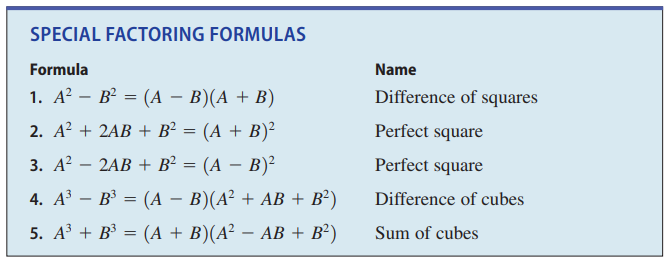
\includegraphics[width=1.1\textwidth]{algebra-pre-calculus/algebraic-expressions/special_factoring_formulas.png}
\end{align*} \break

When we factor an expression, the result can sometimes be factored further. In general, we first factor out common factors, then inspect the result to see whether it can be
factored by any of the other methods of this section. We repeat this process until we
have factored the expression completely

\subsection{Factoring Expressions with Fractional Exponents}
Factor each expresson. \\ \break
\textbf{(a)} \scalebox{1.2}{$3x^{\frac{3}{2}}-9x^{\frac{1}{2}}+6x^{-\frac{1}{2}}$ = $3x^{-\frac{1}{2}}(x^2-3x+2)$ = $3x^{-\frac{1}{2}}(x-2)(x-1)$} \\ \break
Here we have taken the common factor $3x^{-\frac{1}{2}}$ out of each term. Then we have factored the quadratic expression $x^2-3x+2$. \\ \break

\textbf{(b)} $(2+x)^{-\frac{2}{3}}x+(2+x)^{\frac{1}{3}} = (2+x)^{-\frac{2}{3}}[x+(2+x)] = (2+x)^{-\frac{2}{3}}(x+2+x) = (2+x)^{-\frac{2}{3}}(2x+2)$ \\ \break
Here we have taken the common factor $(2+x)^{-\frac{2}{3}}$ out of each term. Then we have just simplified. \\ \break % Section 4 - Algebraic Expressions
\section{Rational Expressions}
A quotient of two algebraic expressions is called a \textbf{fractional expression}. Here are
some examples:
$$ \frac{2x}{x-1} \quad \frac{y-2}{y^2+4} \quad \frac{x^3-x}{x^2+5x+6} \quad \frac{x}{\sqrt{x^2+1}}$$

A \textbf{rational expression} is a fractional expression in which both the numerator and the
denominator are polynomials. For example, the first three expressions in the above
list are rational expressions, but the fourth is not, since its denominator contains a
radical. In this section we learn how to perform algebraic operations on rational expressions.

\subsection{The Domain fo an Algebraic Expression}
In general, an algebraic expression may not be defined for all values of the variable.
The \textbf{domain} of an algebraic expression is the set of real numbers that the variable is
permitted to have. The table in the margin gives some basic expressions and their
domains

\begin{align*}
    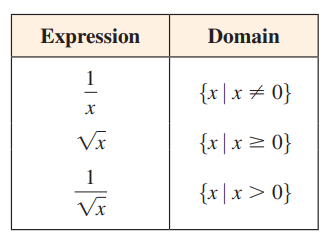
\includegraphics{algebra-pre-calculus/rational-expressions/expressions_domain.png}
\end{align*}

\subsection{Finding the Domain of an Expression}
Find the domains of the following expressions:
\textbf{(a)} $2x^2+3x-1$
This polynomial is defined for every x. Thus the domain is the set $\mathbb{R}$ of real
numbers. \\
\textbf{(b)} $\displaystyle \frac{x}{x^2-5x+6}$ \quad $\rightarrow$ We first factor the denominator. 
$$ x^2-5x+6 = (x-2)(x-3)$$ Since the denominator is zero when $x=2$ or $x=3$, the domain is the set of all real numbers except 2 and 3. So: $$ \text{Domain} = \{ x \in \mathbb{R} \mid x \neq 2, 3 \}$$
\\ \break 
\textbf{(c)} $\displaystyle \frac{\sqrt{x}}{x-5}$ \quad $\rightarrow$ For the numerator to b e defined, we must have $x\geq0$. Also we cannot we divide by zero, so $x\neq5$
Thus the domain is the set of all real numbers greater than or equal to zero, except 5. So: $$ \text{Domain} = \{ x \in \mathbb{R} \mid x \geq 0, x \neq 5 \}$$

\subsection{Simplifying Rational Expressions}
To \textbf{simplify rational expressions}, we factor both the numerator and the denominator and then \textbf{cancel} common factors from the numerator and denominator.
Like: $$ \frac{x^2-1}{x^2+x-2} = \frac{\cancel{(x-1)}(x+1)}{\cancel{(x-1)}(x-2)}=\frac{x+1}{x-2}$$


\subsection{Multiplying and Dividing Rational Expressions}
To \textbf{multiply rational expressions}, we are multiplying the numerators and denominators together. Like: $$ \frac{2x}{x^2-1} \cdot \frac{x^2-1}{x^2+1} = \frac{2x(x^2-1)}{(x^2-1)(x^2+1)} = \frac{2x}{x^2+1}$$ 

When it comes to \textbf{divide rational expressions}, we are multiplying the numerator by the reciprocal of the denominator. Like: $$ \frac{2x}{x^2-1} \div \frac{x^2-1}{x^2+1} = \frac{2x}{x^2-1} \cdot \frac{x^2+1}{x^2-1} = \frac{2x(x^2+1)}{(x^2-1)(x^2+1)} = \frac{2x}{x^2-1}$$

\subsection{Adding and Subtracting Rational Expressions}
To \textbf{add or subtract rational expressions}, we need to find a common denominator. We can do this by finding the least common multiple of the denominators. Like: $$ \frac{2}{x-1} + \frac{3}{x+1} = \frac{2(x+1)}{(x-1)(x+1)} + \frac{3(x-1)}{(x-1)(x+1)} = \frac{2x+2}{(x-1)(x+1)} + \frac{3x-3}{(x-1)(x+1)} = \frac{5x-1}{(x-1)(x+1)}$$

\subsection{Rationalizing the denominator or the Numerator}
If a fraction has a denominator of the form $A+B\sqrt{C}$, we can rationalize the denominator by multiplying numerator and denominator by the conjugate radical(its opposite) $A-B\sqrt{C}$.
This works because, by Special Product Formula 1, the product of the
denominator and its conjugate radical does not contain a radical:

$$ (A+B\sqrt{C})(A-B\sqrt{C})=A^2-B^2C$$

\subsection{Rationalizing the Denominator}
Rationalise the denominator: $\displaystyle \frac{1}{1+\sqrt{2}}$ \\ \break
We can multiply the numerator and denominator by the conjugate radical $1-\sqrt{2}$:
$$ \frac{1}{1+\sqrt{2}} \cdot \frac{1-\sqrt{2}}{1-\sqrt{2}} = \frac{1-\sqrt{2}}{1^2-(\sqrt{2})^2} = \frac{1-\sqrt{2}}{1-2} = \frac{1-\sqrt{2}}{-1} = \sqrt{2}-1$$
Here what we did is that we multiplied the numerator and denominator by the conjugate radical $1-\sqrt{2}$, then we simplified the denominator by using the Special Product Formula 1, and then we simplified the fraction.


\subsection{Rationalizing the Numerator}

Rationalise the numerator: $\displaystyle \frac{\sqrt{4+h}-2}{h}$ \\ \break
We can multiply the numerator and denominator by the conjugate radical $\sqrt{4+h}+2$:
$$ \frac{\sqrt{4+h}-2}{h} \cdot \frac{\sqrt{4+h}+2}{\sqrt{4+h}+2} = \frac{(\sqrt{4+h})^2-2^2}{h(\sqrt{4+h}+2)} = \frac{4+h-4}{h(\sqrt{4+h}+2)} = \frac{h}{h(\sqrt{4+h}+2)} = \frac{1}{\sqrt{4+h}+2}$$
Here what we did is that we multiplied the numerator and denominator by the conjugate radical $\sqrt{4+h}+2$, then we simplified the numerator by using the Special Product Formula 1, and then we simplified the fraction.


\subsection{Avoid Common Errors}
Don’t make the mistake of applying properties of multiplication to the operation of addition.
Many of the common errors in algebra involve doing just that. The following table states
several properties of multiplication and illustrates the error in applying them to addition.

\begin{align*}
    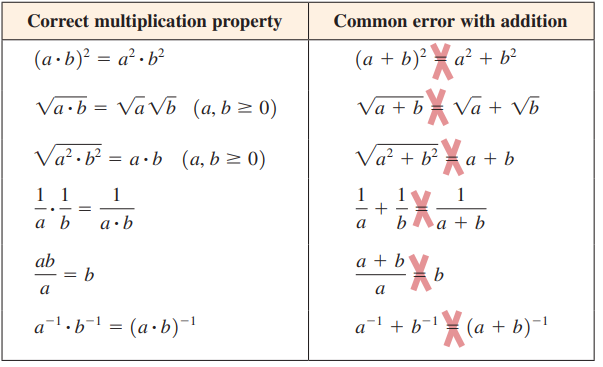
\includegraphics{algebra-pre-calculus/rational-expressions/common_errors.png}
\end{align*}

To verify that the equations in the right-hand column are wrong, simply substitute
numbers for a and b and calculate each side. % Section 5 - Rational Expressions
\section{Factorials}
In mathematics, the factorial of a non-negative integer(whole number (not a fractional number) that can be positive, negative, or zero.) $ n $, denoted by $ n! $, is the product of all positive integers less than or equal to $ n $ \\

$$ 5! = 5 \cdot 4 \cdot 3 \cdot 2 \cdot 1 = 123 $$ \\
Generically expressing, 
$$ n! = n \cdot (n-1) \cdot (n-2) \cdot (n-3) \cdot ... \cdot 3 \cdot 2 \cdot 1 $$

\subsection{Operations with factorials}
Let's clarify a couple of easy examples, 
$$ 2! + 3! = 2 \cdot 1 + 3 \cdot 2 \cdot 1 = 8 $$ 
$$ 3! 4! = 3 \cdot 2 \cdot 1 \cdot 4 \cdot 3 \cdot 2 \cdot 1 = 144 $$ \
When it comes to a fraction of factorials there are some tricks to implement: 
$$ \frac{9!}{7!} = \frac{9 \cdot 8 \cdot 7!}{7!} = 9 \cdot 8 = 72$$
Since, $ 7! = 7 \cdot 6 \cdot 5 \cdot 4 \cdot 3 \cdot 2\cdot 1 $ \\
Consider a similar example: 
$$ \frac{4!5!}{6!} = \frac{(4 \cdot 3 \cdot 2 \cdot 1)(5!)}{6 \cdot 5!} = \frac{24}{6} = 4 $$ \\ 
Also make sure to note these rules:
$$ a! \cdot b! \neq (a + b)! $$ 

This rule applies for addition, subtraction, and division as well. 
So, 
$$ (a!)(b!) \neq (a+b)! $$
$$ \frac{(a!)}{(b!)} \neq (a-b)! $$
$$ (a!) - (b!) \neq (a-b)! $$

\subsection{Algebraic Expressions with factorial}
When dealing with different concepts it is always very important to establish generic / general equations. \\ 
For example let's consider this equation:
$$ \frac{(n+1)!}{n!} = n+1 $$ 

In order to prove this equation there can be two different approaches.
\subsubsection{Proof 1 - Easier and more genuine way of proving it}
This way is the easier way but this doesn’t prove it algebraically/mathematically it just only takes two example and assume that the general equation \textbf{must} be true. 
$$ \frac{(n+1)!}{n!} = n+1 $$
$$ \frac{8!}{7!} = \frac{8 \cdot \cancel{7!}}{\cancel{7!}} = 8 $$
This very easily proves it, however when dealing with research or more advanced mathematics this is not a valid proof. Everything has to be proved algebraically and mathematically.

\subsubsection{Proof 2 - Mathematically proven}
Before seeing the actual proof equation, let's establish a general equation for factorial.
$$ (n+1)! = (n+1) \cdot n! $$
This is true because of the definition of factorial. \\ Meaning that $ (n+1)! = (n+1) \cdot n \cdot (n-1) \cdot (n-2) \cdot ... \cdot 3 \cdot 2 \cdot 1 $ \\
Therefore, 
$$ \frac{(n+1)!}{n!} = \frac{(n+1) \cdot \cancel{n!}}{\cancel{n!}} = n+1 $$
With subtraction,
$$ \frac{(n-1)!}{n!} = \frac{\cancel{(n-1)!}}{n \cdot \cancel{(n-1)!}} = \frac{1}{n} $$

Obviously, different numbers could have been used other than $ 1 $. 
So for example,
$$ \frac{(n+2)!}{n!} = \frac{(n+2) \cdot (n+1) \cdot \cancel{(n)!} }{\cancel{n!}} = (n+2)(n+1) $$
$$ \frac{(2n + 1)!}{(2n)!}  = \frac{(2n + 1) \cdot \cancel{(2n)!}}{\cancel{(2n)!}} = 2n + 1 $$

With this in mind, working with factorials algebraically shouldn't cause any problem. 

\subsection{Other use case of factorial}
Factorial can be used in many different ways. For example in probability, it can be used for combinations. Let's say that we have four different colours and we have to choose four of them. How many different combinations can we have? 
$$ 4! = 4 \cdot 3 \cdot 2 \cdot 1 = 24$$ % Section 6 - Factorials
\section{Intervals}

In mathematics, intervals are a fundamental concept used to represent sets of real numbers. They are commonly used to describe domains of functions, solutions to inequalities, and other mathematical concepts. Intervals come in several forms, each with its own notation and meaning.

\subsection{Open Interval: $(a, b)$}

An open interval between two numbers, $a$ and $b$, is represented as $(a, b)$. It includes all real numbers greater than $a$ and less than $b$, excluding the endpoints $a$ and $b$ themselves. In mathematical notation, this can be expressed as:

$$(a, b) = \{x \in \mathbb{R} \mid a < x < b\}$$

For example, $(1, 3)$ represents all real numbers greater than 1 and less than 3, but it does not include 1 and 3.

\subsection{Closed Interval: $[a, b]$}

A closed interval between two numbers, $a$ and $b$, is represented as $[a, b]$. It includes all real numbers greater than or equal to $a$ and less than or equal to $b$, including the endpoints $a$ and $b$. In mathematical notation, this can be expressed as:

$$[a, b] = \{x \in \mathbb{R} \mid a \leq x \leq b\}$$

For example, $[1, 3]$ represents all real numbers greater than or equal to 1 and less than or equal to 3, including 1 and 3.

\subsection{Half-Open or Half-Closed Intervals: $[a, b)$ and $(a, b]$}

Half-open or half-closed intervals are intervals that include one endpoint but not the other. They are represented as $[a, b)$ and $(a, b]$.

- $[a, b)$ includes all real numbers greater than or equal to $a$ and less than $b$, including $a$ but not $b$.
- $(a, b]$ includes all real numbers greater than $a$ and less than or equal to $b$, including $b$ but not $a$.

For example, $[1, 3)$ represents all real numbers greater than or equal to 1 and less than 3, including 1 but not 3. $(1, 3]$ represents all real numbers greater than 1 and less than or equal to 3, including 3 but not 1.

\subsection{Infinite Intervals: $(-\infty, a)$ and $(a, \infty)$}

Infinite intervals are used to represent unbounded sets of real numbers. They are represented as $(-\infty, a)$ and $(a, \infty)$.

- $(-\infty, a)$ includes all real numbers less than $a$.
- $(a, \infty)$ includes all real numbers greater than $a$.

For example, $(-\infty, 1)$ represents all real numbers less than 1 (negative infinity to 1), and $(1, \infty)$ represents all real numbers greater than 1 (1 to positive infinity).

\subsection{Combining Intervals: Union ($\cup$)}

You can combine multiple intervals using the union symbol ($\cup$) to represent a domain that includes multiple disjoint intervals. For example, if you have the intervals $(1, 3)$ and $(5, 7)$, their union is represented as $(1, 3) \cup (5, 7)$, which includes all real numbers between 1 and 3 (excluding 1 and 3) and all real numbers between 5 and 7 (excluding 5 and 7).

In summary, intervals are a powerful tool in mathematics for representing sets of real numbers. Understanding the different types of intervals and their notations is essential for working with functions, inequalities, and various mathematical concepts.
 % Section 7 - Intervals
\section{Factoring}
In mathematics, factorization or factoring consists of writing a number or another mathematical object as a product of several factors, usually smaller or simpler objects of the same kind. \\

\subsection{Factoring by pulling out HCF}

The first method of factoring is by pulling out the highest common factor often referred as “HCF”. 

\begin{align*}
    &A. \quad 15 + 25x = 5(3 + 5x) \\
    &B. \quad x^2y + y^2x^3 = x^2y(1 + xy) \\
\end{align*}

You can always check whether you have factored correctly by expanding the brackets.

\subsection{Factoring by grouping}
Second method of factoring is factoring by grouping, in this method we are looking for more terms, generally at least 4 terms. We are grouping the terms together in pairs of two terms so that each pair of terms has a common factor that we can factor out. 

\begin{align*}
    A. \quad x^3 + 3x^2 + 4x + 12 &= x^2(x + 3) + 4(x + 3) = (x^2 + 4)(x + 3) \\
\end{align*}

Notice that once we factored out the common factor, we were left with a common binomial factor. We can factor out the common binomial factor to get the final answer.

\subsection{Factoring quadratics}
A quadratic is an expression with a squared term, then just a term with a variable, then a constant. 
\\ Like this: $ax^2 + bx + c$ 

We are looking for two numbers that multiply you get $c$ and when you add them you get $b$.
The reason why: 
$$ (x + m)(x + n) = \\ x^2 + mx + nx + mn = x^2 + \underbrace{(m + n)}_b x + \underbrace{(mn)}_c $$

$m$ and $n$ are the two numbers we are looking for. As you can see $m + n = b$ and $mn = c$. \\

\textbf{Example}. Factor $x^2 - 6x + 8$ \\
We are looking for two numbers that multiply you get $8$ and when you add them you get $-6$. \\
The two numbers are $-2$ and $-4$ because $-2 \cdot -4 = 8$ and $-2 + -4 = -6$. \\
Therefore, 
\begin{align*}
    x^2 - 6x + 8 &= (x - 2)(x - 4) \\
\end{align*}

\textbf{Example}. Factor $10x^2 + 11x - 6$ \\
\begin{itemize}
    \item Step 1. Multiply the leading coefficient (10) and the constant term (-6) to get -60. \\
    \textbf{Why?} The main goal in factoring a quadratic equation is to express it as the product of two binomials(like (2x+4)(4x+5)). 
    In the case of a quadratic with a leading coefficient (the coefficient of $x^2$) not equal to 1, like $10x^2$ in our example, we need to find two binomials of the form $(ax + b)(cx + d)$ e.g $(2x + 4)(5x+2)$ such that their product equals the given quadratic. 
    So, in this context, we are essentially trying to break down the original quadratic ($10x^2 - 11x - 6$) into two binomials, and we start by looking for two numbers that will help us achieve this. These two numbers should meet two criteria:
    \begin{itemize}
        \item Their product should equal the product of the leading coefficient and the constant term (in this case, $10 \cdot -6 = -60$).
        \item Their sum should equal the coefficient of the x-term (in this case, -11)
    \end{itemize}
    By finding such numbers, we can rewrite the middle term of the quadratic equation (the -11x term) as the sum or difference of two terms, each of which can be factored more easily. This allows us to perform factoring by grouping, making the overall factoring process more manageable.
    \item Step 2.  Find two numbers that multiply to -60 and add up to the coefficient of the x-term (-11). In this case, those two numbers are -15 and 4 because $(-15) \cdot 4 = -60$ and $(-15) + 4 = -11$.
    \item Step 3. Rewrite the middle term (-11x) using the two numbers found in step 2: 
    $$ 10x^2 - 15x + 4x - 6 $$
    \item Step 4. Group the terms: Group the first two terms $(10x^2 - 15x)$ and the last two terms $(4x - 6)$. This will gve us: 
    $$ 5x(2x - 3) + 2(2x - 3) $$
    \item Step 5. Factor out the HCF of each group: 
    $$ 5x(2x - 3) + 2(2x - 3) = (5x + 2)(2x - 3) $$

\end{itemize}
And we are done factorising the quadratic equation.

\subsection{Difference of squares}
The difference of squares is a squared term minus another squared term.
\\ Like this: $a^2 - b^2 = (a+b)(a-b) = a^2-ab+ab-b^2 $ 

\textbf{Example.} Factor $x^2 - 9$ 
$$ (x+3)(x-3) $$


\textbf{Example.} Factor $9p^2 - 1$ 
$$ (3p+1)(3p-1) $$

\subsection{Difference or sum of cubes}
The difference or sum of cubes is a cubed term plus or minus another cubed term.

$$ a^3 - b^3 = (a-b)(a^2+ab+b^2) $$ Because, $$(a-b)(a^2+ab+b^2) = a^3 - ab^2 + a^2b - ab^2 + b^3 = a^3 - 2ab^2 + b^3 $$ 

And, 
$$ a^3 + b^3 = (a+b)(a^2-ab+b^2) $$ Because, $$(a+b)(a^2-ab+b^2) = a^3 + ab^2 - a^2b + ab^2 + b^3 = a^3 + 2ab^2 + b^3 $$ 
\\
\textbf{Example.} Factor $x^3 - 8$ \\
We know that $x^3 - 8 = x^3 - 2^3$
Therefore,
$$ (x-2)(x^2+2x+4) $$

if we expand out: 
$$ (x-2)(x^2+2x+4) = x^3 + 2x^2 + 4x - 2x^2 - 4x - 8 = x^3 - 8 $$
Therefore our answer is correct.

\subsection{Additional examples of factoring}
\textbf{Example.} Which of these expressions DOES NOT factorise?

A. $x^2 + x$ \\
This can be factored by pulling out the highest common factor. \\
$$ x^2 + x = x(x+1) $$

B. $x^2 - 25$ \\
This also can be factored by difference of squares. \\
$$ x^2 - 25 = (x+5)(x-5) $$

C. $x^2 + 4$ \\
This cannot be factored because it is a sum of squares not a difference of squares. \\

D. $x^3+2x^2+3x+6$ \\
This can also be factored by grouping. \\
$$ x^3+2x^2+3x+6 = x^2(x+2)+3(x+2) = (x^2+3)(x+2) $$

E. $5x^2-14x+8$ \\
This can also be factored by using the method of factoring quadratics when $a \neq 1$. \\
Therefore we can multiply the leading coefficient (5) and the constant term (8) to get 40. \\
We are looking for two numbers that multiply you get 40 and when you add them you get -14 and those are -10 and -4. \\
So we can rewrite the middle term (-14x) using the two numbers found:
$$ 5x^2 - 10x - 4x + 8 $$ 
Then we can group them together:
$$ 5x(x - 2) - 4(x - 2) $$
And finally factor out the HCF of each group:
$$ (5x - 4)(x - 2) $$

Eventually the answer for our question is C. $x^2 + 4$ because it cannot be factored.

\subsection{Tips and Extra examples}
\begin{itemize}
    \item Always look for the highest common factor first. That will simplify things and make the rest of the factoring more easier. 
    \item You might need to do several steps of factoring to get the final answer. For example you might have to pull out the HCF first then you can do factoring by grouping or factoring quadratics. Then you might also apply difference of squares or difference or sum of cubes. Keep factoring as far as you can go.
\end{itemize}

\textbf{Extra Example} Factor $2z^2 + 3z -14$ \\
Again as previously done first we need to multiply the leading coefficient (2) and the constant term (-14) to get -28. \\ 
We are looking for two numbers that multiply you get -28 and when you add them you get 3 and those are 7 and -4. \\
So we can rewrite the middle term (3z) using the two numbers found:
$$ 2z^2 + 7z - 4z - 14 $$ 
Then we can group them together:
$$ z(2z + 7) - 2(2z + 7) $$
And finally factor out the HCF of each group:
$$ (z - 2)(2z + 7) $$

\textbf{Extra Example} Factor $-5v^2-45v+50$ \\
Again as previously done first we need to multiply the leading coefficient (-5) and the constant term (50) to get -250. \\
We are looking for two numbers that multiply you get -250 and when you add them you get -45 and those are -50 and 5. \\
So we can rewrite the middle term (-45v) using the two numbers found:
$$ -5v^2 - 50v + 5v + 50 $$ 
Then we can group them together:
$$ -5v(v + 10) + 5(v + 10) $$
And finally factor out the HCF of each group:
$$ (-5v + 5)(v + 10) $$
This can be further simplified to:
$$ -5(v - 1)(v + 10) $$
Another solution for this could have been that first we could have pulled out the HCF which is -5 and then we could have factored the quadratic. \\
$$ -5v^2 - 45v + 50 = -5(v^2 + 9v - 10) $$
And this is really easy since $ a = 1 $ Therefore we need two numbers that multiply you get -10 and when you add them you get 9 and those are 10 and -1. \\
So we can say that: 
$$ -5(v^2 + 9v - 10) = -5(v + 10)(v - 1) $$ % Section 8 - Factoring
\section{Equations}
An equation is a statement that two mathematical expressions are equal. For example,
\begin{equation}
    2x + 3 = 5
\end{equation}

the letter $x$ is the variable. We think of $x$ as the “unknown” in the equation, and our goal
is to find the value of $x$ that makes the equation true. The values of the unknown that
make the equation true are called the \textbf{solutions} or \textbf{roots} of the equation, and the process
of finding the solutions is called \textbf{solving the equation}. \\

Two equations with exactly the same solutions are called \textbf{equivalent equations}. To
solve an equation, we try to find a simpler, equivalent equation in which the variable
stands alone on one side of the “equal” sign. Here are the properties that we use to solve
an equation. (In these properties, $A$, $B$, and $C$ stand for any algebraic expressions, and
the symbol 3 means “is equivalent to.”)

\begin{align*}
    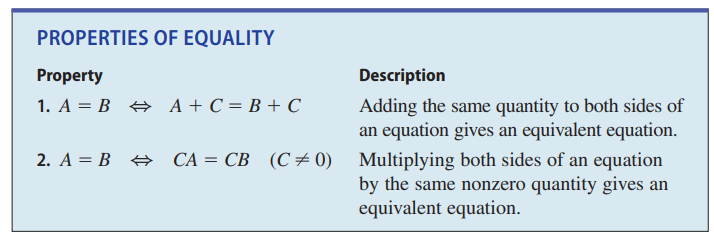
\includegraphics[width=1.1\textwidth]{algebra-pre-calculus/equations/properties_of_equations.png}
\end{align*}


\section{Solving Quadratic Equations}
\label{sec:quadratic-equations}
A quadratic equation is an equation that's highest exponent/power is 2. It can be written in the form of $ax^2+bx+c=0$ where $a,b,c$ are constants representing real numbers and $a \neq 0$. In this section we will go over how to solve quadratic equations.

\subsection{Solving quadratic equations by factoring}
For example: 
$$ 3x^2+7x-2=0$$ where $a=3$, $b=7$, and $c=-2$.
This also a quadratic equation but not in standard form: 
$$ 3x^2=-7x+2$$

The key to solve quadratic equations is: 
\begin{enumerate}
    \item Write it in standard form.
    \item Factor it or use the quadratic formula.
\end{enumerate}

\textbf{Example}. Find all real solutions for the equation $y^2=18-7y$
First following the steps is to re-write the equation in standard form.
$$y^2+7y-18=0$$
Then as we previously discussed during factoring we need to look for two numbers that multiply to $-18$ and add to $7$. The numbers are $9$ and $-2$.

Therefore, the equation can be factored as:
$$(y+9)(y-2)=0$$
Now for the equation to be true, one of the factors must be equal to zero. Therefore, $y+9=0$ or $y-2=0$. Solving for $y$ we get $y=-9$ or $y=2$. Therefore, the solutions for the equation are $y=-9$ or $y=2$.

You can check whether they are correct by substituting the values of $y$ in the original equation. So:
$$(-9)^2=18-7(-9)$$
$$81=18+63$$ which is true. Therefore, $y=-9$ is a solution.
To check for $y=2$:
$$(2)^2=18-7(2)$$
$$4=18-14$$ which is also true. Therefore, $y=2$ is also a solution.
\newpage
\textbf{Example}. Solve the equation $w^2=121$ \\
First we need to re-write the equation in standard form:
$$w^2-121=0$$ where $a=1$, $b=0$, and $c=-121$.
Then we need to factor the equation. We can factor it as:
$$(w+11)(w-11)=0$$ Because $w^2-121=(w+11)(w-11)$. \\

Again, for the equation to be true, one of the factors must be equal to zero. Therefore, $w+11=0$ or $w-11=0$. Solving for $w$ we get $w=-11$ or $w=11$. Therefore, the solutions for the equation are $w=-11$ or $w=11$.

Now we could have solved the equation by taking the square root of both sides. So:
\begin{align*}
    w^2&=121 \\
    \sqrt{w^2}&=\pm \sqrt{121} \\
    w&=\pm 11
\end{align*}

The reason why we have to take plus and minus is because when we take the square root of both sides we get $w=\pm 11$ because $11^2=121$ and $(-11)^2=121$ as well.

\textbf{Example}. Solve the equation $x(x+2) = 7$
\\
First we need to re-write the equation in standard form by multiplying out and subtracting $7$ from both sides:
$$x^2+2x-7=0$$ where $a=1$, $b=2$, and $c=-7$.
Now again we are looking for two numbers that multiply to $-7$ and add to $2$. Unfortunately, there are no two whole numbers that multiply to $-7$ and add to $2$. Therefore, we can't factor the equation. So we have to use the quadratic formula to solve the equation.
\subsection{Quadratic formula}
The quadratic formula is a formula that gives the solutions for a quadratic equation. In our example $a = 1$, $b = 2$, and $c = -7$. So the quadratic formula is:
$$x=\frac{-b \pm \sqrt{b^2-4ac}}{2a}$$
So plugging in the values of $a$, $b$, and $c$ we get:
$$x=\frac{-2 \pm \sqrt{2^2-4(1)(-7)}}{2(1)}$$

Simplifying we get:
$$x=\frac{-2 \pm \sqrt{32}}{2} = \frac{-2\pm\sqrt{16\cdot2}}{2} = \frac{-2\pm4\sqrt{2}}{2} $$
Simplifying everything we get: 
$$ -1\pm2\sqrt{2} $$
So the solutions are: $x=-1+2\sqrt{2}$ or $x=-1-2\sqrt{2}$.

\textbf{Example}. Solve the equation $\frac{1}{2}y^2 = \frac{1}{3}y-2$ \\

First we need to re-write the equation in standard form by multiplying out and subtracting $\frac{1}{3}y-2$ from both sides:
$$\frac{1}{2}y^2-\frac{1}{3}y+2=0$$ where $a=\frac{1}{2}$, $b=-\frac{1}{3}$, and $c=2$.

Let's get rid of the denominator by multiplying both sides by $6$ which is the least common multiple of $2$ and $3$:
$$3y^2-2y+12=0$$ where $a=3$, $b=-2$, and $c=12$.

Now let's use the quadratic formula to solve the equation:
$$x=\frac{2\pm\sqrt{(-2)^2-4(3)(12)}}{2(3)}$$

Simplifying we get:
$$x=\frac{2\pm\sqrt{4-144}}{6} = \frac{2\pm\sqrt{-140}}{6}$$

Since we cannot square negative numbers this equation has no real solutions. 
The reason why we cannot square negative numbers is because any number squared will produce a positive number, so there is no true square root of a negative number.

The steps to solve quadratic equations are:
\begin{enumerate}
    \item Write the equation in standard form.
    \item Factor the equation or use the quadratic formula. Because factoring is not always possible, but the quadratic formula always works. Therefore, you can't really lose by using the quadratic formula, however sometimes it is easier and faster to factor the equation.
\end{enumerate}

\subsection{Solving quadratic equations by completing the square}
If a quadratic equation does not factor readily, then we can solve it using the technique of \textbf{completing the square}.
This means that we add a constant to an expression to make it a perfect square. For example, to make $x^2-6x$ a perfect square, we must add $9$, since $(x-3)^2=x^2-6x+9$. \\
Being aware of the standard form: $ax^2+bx+c=0$:

\begin{align*}
    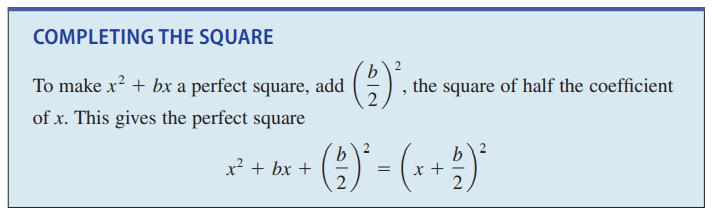
\includegraphics[width=1.3\textwidth]{algebra-pre-calculus/equations/completing_square.png}
\end{align*}

\textbf{(a)} $x^2-8x+13=0$
\textbf{()} % Section 9 - Equations
\section{Solving Radical Equations}
A radical equation is an equation in which a variable is under a radical symbol. The most common radical equations are square root equations, However there can be cube root, 4th root up to nth root which can be any number.

\subsection{Solving Square Root Equations} 
\textbf{Example.} Solve: $x+\sqrt{x} = 12$ \\
When we see an equation with a square root, we just want to get rid of it, the way we do it is we isolate the square root. In other words we want to get the term with the square root in it on one side of the equation and everything else by itself. \\

Therefore, the steps can be
\begin{enumerate}
    \item Isolate the square root 
    \begin{align*}
        x+\sqrt{x} &= 12 \\
        \sqrt{x} &= 12-x \quad \text{(get rid of the square root by squaring both sides)} \\
    \end{align*}
    \item Get rid of the square root. 
    \begin{align*}
        x &= (12-x)^2 \\
        x &= 144 - 24x + x^2 \\
        0 &= x^2 - 25x + 144 \quad \text{(get two numbers that multiply to 144 and app up to -25)} \\ 
    \end{align*}
   \item Solve the quadratic equation
    \begin{align*}
         0 &= x^2 - 25x + 144 \\
         0 &= (x-9)(x-16) \\
         x &= 9, 16
    \end{align*}
    \item Check the answer and eliminate extraneous solutions. 
    \begin{align*}
        x &= 9, 16 \\
        x+\sqrt{x} &= 12 \\
        9+\sqrt{9} &= 12 \\
        9+3 &= 12 \\
        12 &= 12 \quad \text{True} \\
        16+\sqrt{16} &= 12 \\
        16+4 &= 12 \\
        20 &= 12 \quad \text{False} \\
    \end{align*}
    Therefore, the answer is $x=9$.
\end{enumerate}

\textbf{Example.} Solve: $2p^{\frac{4}{5}} = \frac{1}{8}$
You'd might think that this is not a radical equation, however we know that radicals can be rewirtten as fractional exponents. 
Following our steps: 
\begin{enumerate}
    \item Isolate the radical
    \begin{align*}
        2p^{\frac{4}{5}} &= \frac{1}{8} \quad \text{Divide by 2 so we can isolate the radical/fractional exponent} \\
        p^{\frac{4}{5}} &= \frac{1}{16} 
    \end{align*}
    \item Get rid of the radical/fractional exponent.
    Now here we can get raise both sides to the power of $5$. 
    \begin{align*}
        p^{\frac{4}{5}} &= \frac{1}{16} \\
        (p^{\frac{4}{5}})^5 &= \left(\frac{1}{16}\right)^5 \\
        p^4 &= \frac{1}{16^5} \quad \text{Multiply by $\frac{1}{4}$ OR $\sqrt[4]{x^1}$} \\
    \end{align*}
    \item Solve the equation
    \begin{align*}
        (p^4)^{\frac{1}{4}} &= \pm \left(\left(\frac{1}{6}\right)^5\right)^{\frac{1}{4}} \quad \text{Be careful because our answer can be + or - as well} \\ 
        p &= \pm \left(\frac{1}{16}\right)^{\frac{5}{4}} \quad \text{Rewrite this using our fractional exponent rule} \\
        p &= \pm  \left(\sqrt[4]{\frac{1}{16}}\right)^5 \\
        p &= \pm \left(\frac{\sqrt[4]{1}}{\sqrt[4]{16}}\right)^5 \\
        p &= \pm \left(\frac{1}{2}\right)^5 \\
        p &= \pm \frac{1}{32} 
    \end{align*}
    Therefore our answer is $p=\pm \frac{1}{32}$
    \item Check the answer and eliminate extraneous solutions. Let's plug in our answer into the original equation.
    \begin{align*}
        2p^{\frac{4}{5}} &= \frac{1}{8} \\
        2\left(\frac{1}{32}\right)^{\frac{4}{5}} &= \frac{1}{8} \\
        2\left(\frac{1^{\frac{4}{5}}}{32^{\frac{4}{5}}}\right) &= \frac{1}{8} \\
        2\left(\frac{1}{(\sqrt[5]{32})^4}\right) &= \frac{1}{8} \\
        2\left(\frac{1}{16}\right) &= \frac{1}{8} \\
        \frac{1}{8} &= \frac{1}{8} \quad \text{True} \\
    \end{align*}
    We also could have gotten rid of the fractional exponent, by raising both sides to the power of $\frac{5}{4}$.
    So: 
    \begin{align*}
        p^4 &= \frac{1}{16^5} \\
        (p^{\frac{4}{5}})^{\frac{5}{4}} &= \left(\frac{1}{16^5}\right)^{\frac{5}{4}} \\
        p &= (\frac{1}{16})^{\frac{5}{4}} 
    \end{align*}
    And then so on as we did before.
\end{enumerate} % Section 10 - Solving Radical Equations
\section{Absolute Value Inequalities}
\textbf{Example.} What x-values satisfy $|x|<$5? \\
\textbf{Solution.} We can solve this problem by using a number line. We know that the distance between x and 0 is less than 5. So, the x-values that satisfy the inequality are somewhere between -5 to 5. \\
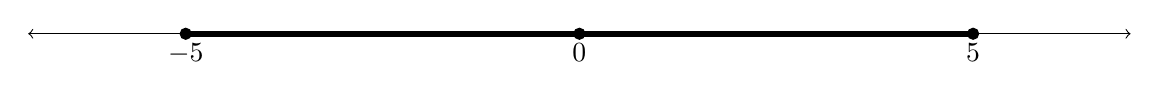
\begin{tikzpicture}
    % Draw the number line
    \draw[<->] (-7,0) -- (7,0);

    % Mark 0
    \draw[fill=black] (0,0) circle (2pt) node[below] {$0$};

    % Mark -5
    \draw[fill=black] (-5,0) circle (2pt) node[below] {$-5$};

    % Mark 5
    \draw[fill=black] (5,0) circle (2pt) node[below] {$5$};

    % Bold line between -5 and 5
    \draw[line width=2pt] (-5,0) -- (5,0);
\end{tikzpicture}
We can express this inequality without using absolute value. We know that $|x|<$5 is equivalent to $-5<x<5$. Because $x$ is somewhere between -5 and 5. Therefore the solution is $-5<x<5$. Or as an interval notation: $(-5,5)$.
\\
\vspace{4pt}
\textbf{Example.} What x-values satisfy $|x|\geq5$? \\
Since $|x|$ has to be greater than or equal to 5, $|x|$ has to be bigger then 5 and -5, since it can be both positive and negative. So, the x-values that satisfy the inequality are somewhere less than -5 or greater than 5. \\
\\
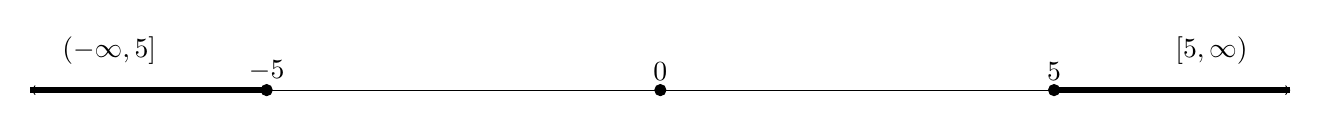
\begin{tikzpicture}
    % Draw the number line
    \draw[<->] (-8,0) -- (8,0);

    % Mark 0, 5, and -5 with filled circles
    \draw[fill=black] (0,0) circle (2pt) node[above] {$0$};
    \draw[fill=black] (5,0) circle (2pt) node[above] {$5$};
    \draw[fill=black] (-5,0) circle (2pt) node[above] {$-5$};

    % Mark the regions to be emphasized with bold lines
    \draw[line width=2pt] (-8,0) -- (-5,0);
    \draw[line width=2pt] (5,0) -- (8,0);

    % Label the emphasized regions
    \node at (-7,0.5) {$(-\infty, 5]$};
    \node at (7,0.5) {$[5, \infty)$};
\end{tikzpicture}

So, $x\leq-5$ or $x\geq5$. Or as an interval notation: $(-\infty, -5]\cup[5, \infty)$.

\textbf{Example.} Solve $|3-2t|<4$. 

Since $|3-2t|$ has to be less than 4 OR bigger -4 we can represent it in a numberline.  \\
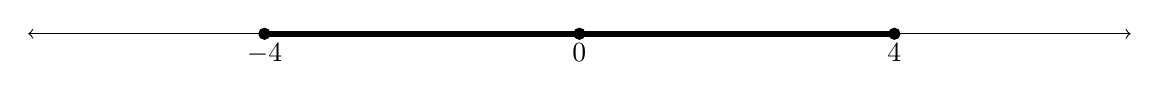
\begin{tikzpicture}
    % Draw the number line
    \draw[<->] (-7,0) -- (7,0);

    % Mark 0
    \draw[fill=black] (0,0) circle (2pt) node[below] {$0$};

    % Mark -5
    \draw[fill=black] (-4,0) circle (2pt) node[below] {$-4$};

    % Mark 5
    \draw[fill=black] (4,0) circle (2pt) node[below] {$4$};

    % Bold line between -5 and 5
    \draw[line width=2pt] (-4,0) -- (4,0);
\end{tikzpicture}

Therefore, we can just have two different equations: 
\begin{align*}
    3-2t<4 \\
    3-2t>-4
\end{align*}
Solving the first equation:
\begin{align*}
    3-2t<4 \\
    -2t<1 \\
    t>-\frac{1}{2}
\end{align*}
Solving the second equation:
\begin{align*}
    3-2t>-4 \\
    -2t>-7 \\
    t<\frac{7}{2}
\end{align*}

In the numberline we can see that the solution is $-\frac{1}{2}<t<\frac{7}{2}$. \\
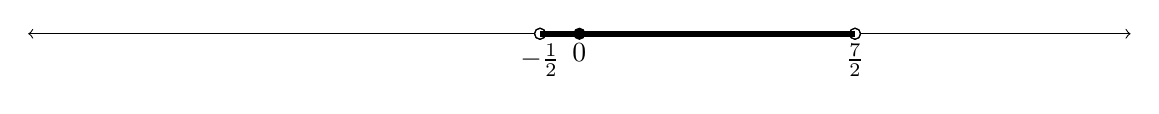
\begin{tikzpicture}
    % Draw the number line
    \draw[<->] (-7,0) -- (7,0);

    % Mark 0
    \draw[fill=black] (0,0) circle (2pt) node[below] {$0$};

    % Mark -1/2 with a hole
    \draw[fill=white] (-1/2,0) circle (2pt) node[below] {$-\frac{1}{2}$};
    \draw (-1/2,0) circle (2pt); % Draw a hole in the circle

    % Mark 7/2 with a hole
    \draw[fill=white] (7/2,0) circle (2pt) node[below] {$\frac{7}{2}$};
    \draw (7/2,0) circle (2pt); % Draw a hole in the circle

    % Bold line between -1/2 and 7/2
    \draw[line width=2pt] (-1/2,0) -- (7/2,0);
\end{tikzpicture}

Or as an interval notation: $(-\frac{1}{2}, \frac{7}{2})$.

Notice that the solution cannot include $-\frac{1}{2}$ and $\frac{7}{2}$ because $|3-2t|$ cannot be equal to 4. % Section 11 - Absolute Value Inequalities
\section{Solving Absolute Value Equations}

The absolute value for a positive number is the number itself. For example, $|3|=3$. The absolute value for a negative number is the number itself with the negative sign removed. For example, $|-3|=3$. The absolute value of a number is always positive or zero. For example, $|0|=0$.
You can think of the absolute value as the distance of a number from zero on the number line. For example, $|3|$ is 3 units away from zero on the number line. $|-3|$ is also 3 units away from zero on the number line. The absolute value of a number is always positive or zero. For example, $|0|$ is 0 units away from zero on the number line.
\\\\
\textbf{Example.} Solve the equation $3|x|+2=4$

\begin{enumerate}
	\item Isolate absolute value part of the equation.
	      \begin{align*}
		      3|x|+2 & =4 \quad \text{Subtract 2 from both sides} \\
		      3|x|   & =2 \quad \text{Divide both sides by 3}     \\
		      |x|    & =\frac{2}{3}
	      \end{align*}
	\item Think in terms of distance. \\
	      \begin{tikzpicture}
		      % Draw the number line
		      \draw[<->] (-3,0) -- (3,0);

		      % Mark 2/3
		      \draw[fill=black] (2/3,0) circle (2pt) node[above] {$\frac{2}{3}$};

		      % Mark 0
		      \draw[fill=black] (0,0) circle (2pt) node[below] {$0$};

		      % Mark -2/3
		      \draw[fill=black] (-2/3,0) circle (2pt) node[below] {$-\frac{2}{3}$};
	      \end{tikzpicture}
	      As we can see from the number line, the distance of $x$ from zero is $\frac{2}{3}$ but since $x$ can be either positive or negative, we have two solutions: $x=\frac{2}{3}$ and $x=-\frac{2}{3}$. Because both solutions are $\frac{2}{3}$ away from zero and their absolute value is the same, we can write the solution as $x=\pm\frac{2}{3}$.
	\item  Check the solution. \\
	      \begin{align*}
		      3|x|+2                      & =4 \quad \text{Substitute $x=\frac{2}{3}$} \\
		      3\left|\frac{2}{3}\right|+2 & =4 \quad \text{Simplify}                   \\
		      3\left(\frac{2}{3}\right)+2 & =4 \quad \text{Simplify}                   \\
		      2+2                         & =4 \quad \text{Simplify}                   \\
		      4                           & =4 \quad \text{True}
	      \end{align*}
	      Let's plug in $x=-\frac{2}{3}$.
	      \begin{align*}
		      3|x|+2                       & =4 \quad \text{Substitute $x=-\frac{2}{3}$} \\
		      3\left|-\frac{2}{3}\right|+2 & =4 \quad \text{Simplify}                    \\
		      3\left(\frac{2}{3}\right)+2  & =4 \quad \text{Simplify}                    \\
		      2+2                          & =4 \quad \text{Simplify}                    \\
		      4                            & =4 \quad \text{True}
	      \end{align*}
	      In conlusion, regardless of the sign of a number that absolute value will always be positive or zero. When solving absolute value equations, you will always get two solutions or no solutions.
\end{enumerate}

\textbf{Example.} Solve the equation $|3x+2|=4$
Let's go through this following the same steps as the previous example.
\begin{enumerate}
	\item Isolate absolute value part of the equation.
	      The absolute value part of the equation is already isolated.
	\item Think in terms of distance.
	      Since we know that $|3x+2|$ supposed to be at a distance of 4 from zero. Therefore, since it is absolute value it can be either 4 units to the right or 4 units to the left of zero.
	      \\
	      \begin{tikzpicture}
		      % Draw the number line
		      \draw[<->] (-6,0) -- (6,0);

		      % Mark -4
		      \draw[fill=black] (-4,0) circle (2pt) node[below] {$-4$};
		      \node[below] at (-4,-0.5) {$|3x + 2|$};

		      \draw[fill=black] (0,0) circle (2pt) node[below] {$0$};

		      % Mark 4
		      \draw[fill=black] (4,0) circle (2pt) node[below] {$4$};
		      \node[below] at (4,-0.5) {$|3x + 2|$};
	      \end{tikzpicture}
	      \\
	      Therefore, we can write them as two equations:
	      \begin{align*}
		      3x+2 & =4 \quad \text{Solve for $x$}  \\
		      3x   & =2                             \\
		      x    & =\frac{2}{3}                   \\
		      3x+2 & =-4 \quad \text{Solve for $x$} \\
		      3x   & =-6                            \\
		      x    & =-2
	      \end{align*}
	\item Check the solution.
	      \begin{align*}
		      |3x+2|                        & =4 \quad \text{Substitute $x=\frac{2}{3}$} \\
		      |3\left(\frac{2}{3}\right)+2| & =4 \quad \text{Simplify}                   \\
		      |2+2|                         & =4 \quad \text{Simplify}                   \\
		      |4|                           & =4 \quad \text{Simplify}                   \\
		      4                             & =4 \quad \text{True}
	      \end{align*}
	      Let's plug in $x=-2$.
	      \begin{align*}
		      |3x+2|    & =4 \quad \text{Substitute $x=-2$} \\
		      |3(-2)+2| & =4 \quad \text{Simplify}          \\
		      |-6+2|    & =4 \quad \text{Simplify}          \\
		      |-4|      & =4 \quad \text{Simplify}          \\
		      4         & =4 \quad \text{True}
	      \end{align*}
\end{enumerate}

\textbf{Example.} Solve the equation $5|4p-3|+16=1$
Let's go through this following the same steps as the previous example.
\begin{enumerate}
	\item Isolate the absolute value part of the equation.
	      \begin{align*}
		      5|4p-3|+16 & =1 \quad \text{Subtract 16 from both sides} \\
		      5|4p-3|    & =-15 \quad \text{Divide both sides by 5}    \\
		      |4p-3|     & =-3
	      \end{align*}
	\item Think in terms of distance.
	      The problem here is that we can't have a negative distance. An absolute value of a number is always positive or zero. Therefore, there is no solution to this equation.
\end{enumerate} % Section 12 - Solving Absolute Value Equations
\section{Solving Rational Equations}
A Rational equation is an equation that contains one or more rational expressions. A rational expression is a fraction whose numerator and denominator are polynomials. For example, $\frac{x^2+1}{x+1}$ is a rational expression as discussed in the previous section. In this section we will go over how to solve rational equations.

\subsection{Solving Rational Equations}

\textbf{Example.} Solve: $\frac{x}{x+3} = 1+\frac{1}{x}$

The steps to solve a rational equation are as follows:
\begin{enumerate}
    \item Find the least common denominator (LCD) of all the fractions in the equation. In our example we have two fractions, $\frac{x}{x+3}$ and $\frac{1}{x}$, we can think of 1 as $\frac{1}{1}$. \\
    By multiplying them together, therefore the LCD is $(x+3)x$.
    \item Next step is to "clean" the denaminator  by multiplying both sides of the equation by the LCD. So:
    $$ (x+3)x \cdot \frac{x}{x+3} = (x+3)x \cdot \left(1+\frac{1}{x}\right)$$
    The right side of the equation can be simplified as:
    $$ (x+3)x \cdot \left(1+\frac{1}{x}\right) = (x+3)x + (x+3)$$
    Therefore we can rewrite the equation as:
    $$ \cancel{(x+3)}x \cdot \frac{x}{\cancel{x+3}} =  (x+3)x + (x+3)$$
    $$ x^2 =  (x+3)x + (x+3)$$
    \item Third step is to simplify and solve. 
    $$ x^2 =  x^2+3x+x+3$$
    $$ \cancel{x^2} =  \cancel{x^2}+3x+x+3$$
    $$0 =  4x+3$$
    $$4x =  -3$$
    $$x =  -\frac{3}{4}$$
    \item It is a good idea to check your answer by plugging it back into the original equation. In our example after plugging it in, we have:
    $$ \frac{-\frac{3}{4}}{-\frac{3}{4}+3} = 1+\frac{1}{-\frac{3}{4}}$$
    $$ \frac{-\frac{3}{4}}{\frac{9}{4}} = 1-\frac{4}{3}$$
    $$ -\frac{3}{9} = -\frac{1}{3} $$
    Therefore we can conclude that our answer is correct. Our final answer is $x = -\frac{3}{4}$.
\end{enumerate}


\textbf{Example.} Solve: 
\begin{equation*}
    \frac{4c}{c-5} - \frac{1}{c+1} = \frac{3c^2+3}{c^2-4c-5}
\end{equation*}

The steps are the same: 
\begin{enumerate}
    \item Find the LCD of all the fractions in the equation. In our example we have three fractions, $\displaystyle \frac{4c}{c-5}$, $\displaystyle  \frac{1}{c+1}$, and $\displaystyle \frac{3c^2+3}{c^2-4c-5}$. when simplifying the 3rd one to $(c-5)(c+1)$ by factoring, the LCD is $(c-5)(c+1)$.
    \item Next step is to "clean" the denaminator  by multiplying both sides of the equation by the LCD. So:
    $$ (c-5)(c+1) \cdot \frac{4c}{c-5} - (c-5)(c+1) \cdot \frac{1}{c+1} = (c-5)(c+1) \cdot \frac{(3c^2+3)}{(c-5)(c+1)}$$
    Cancelling them we have:
    $$ \cancel{(c-5)}(c+1) \cdot \frac{4c}{\cancel{c-5}} - (c-5)\cancel{(c+1)} \cdot \frac{1}{\cancel{c+1}} = \cancel{(c-5)}\cancel{(c+1)} \cdot \frac{(3c^2+3)}{\cancel{(c-5)}\cancel{(c+1)}}$$
    \item Third step is to simplify and solve So: 
    $$ 4c(c+1) - (c-5) = 3c^2+3$$
    Let's expand the left side of the equation:
    $$ 4c^2+4c - c + 5 = 3c^2+3$$
    After subtracting $3c^2$ and simplifying we have:
    $$ c^2+3c+5 = 3$$
    $$ c^2+3c+2 = 0$$
    Here we are with a quadratic equation, that we can solve by using what we have learned. 
    So we are looking for two numbers that multiply to 2 and add to 3. The numbers are 1 and 2. So we can factor the equation as:
    $$ (c+1)(c+2) = 0$$
    Since either $c+1$ or $c+2$ is equal to 0, we have two solutions: $c = -1$ and $c = -2$.
    \item When we are check our answer by plugging it back into the original equation, we notice that $c=-1$ is not a solution. Because it makes the denominator of the second fraction equal to 0. This is what we call an \textbf{extraneous solution}(In mathematics, an extraneous solution is a solution, such as that to an equation, that emerges from the process of solving the problem but is not a valid solution to the problem).
    Therefore our final answer is $c = -2$.
\end{enumerate}
The steps to solve a rational equation are as follows:
\begin{enumerate}
    \item Find the least common denominator (LCD) of all the fractions in the equation. 
    \item Then "clear" the equation of fractions by multiplying both sides of the equation by the LCD.
    \item  Simplify and solve.
    \item Check your answer by plugging it back into the original equation and eliminate any extraneous solutions(make the denaminator 0).
\end{enumerate} % Section 13 - Solving Rational Equations




\section{Summations}
In mathematics, summation is the addition of a sequence of any kind of numbers, called addends or summands; the result is their sum or total. 
Let's say that we have a sequence of numbers and we want to add them up.

\subsubsection{Summation notation - Sigma notation}
$$  \sum_{i=1}^{n} a_i = a_1 + a_2 + a_3 + \ldots + a_n $$
\begin{itemize}
  \item $ i $ = index of summation
  \item $ n $ = upper limit of summation
\end{itemize}
To understand this let's consider this: 
$$ \sum_{i=1}^{4} i = 1 + 2 + 3 + 4$$
\begin{itemize}
  \item $ i = 1 $, $ i $ is the index of summation, meaning that the number where the summation starts from(in this case $ i = 1 $ so $1$).
  \item $ 4 $ is the upper limit of summation, meaning that the number where the summation ends at(in this case $ 4 $). It is important to note that the upper limit only indicates the limit for the index $i$ and doesn't indicate the number of terms that will be included in the summation.
  \item $ i $ is the formula/rule of summation. Meaning that an expression that will be used in our sequence of numbers. Quite literally the expression that will be used in the summation. This can be as complex as we would like it to be.
\end{itemize}

Let's break down the steps of the summation notation:
\begin{itemize}
  \item Firstly we start at whatever the index is, in this case it is $1$ so we start from there. 
  \item Set $i$ equal to one and then write the $1$ down. 
  \item Then we increment the index $i$, and again writing $i$ down and then summing each of these terms as we go.
  \item We continue this process until we reach the upper limit of summation, in this case it is $4$.
  \item Finally we add up all of the terms that we wrote down.
\end{itemize}

\subsubsection{Examples}
Let's consider these examples:
$$ \sum_{i = 1}^{50} \pi \cdot i^2  = \pi0^2 + \pi1^2 + \pi2^2 + \ldots + \pi(50)^2$$
$$ \sum_{i = 0}^{3} (i^2 + 2i + 4) = (0 + 0 + 4) + (1+2+4) + (4+4+4) + (9+6+4) = 42$$
$$ \sum_{i = 0}^{3} (3i + 2)^2 = 4+25+63+121 = 214$$
 % Section 14 - Summations
\section{Complex numbers}

From the section \hyperref[sec:equations]{Equations} we saw that if the discriminant of a quadratic equation is negative, the
equation has no real solution. For example, the equation $$x^2+4=0$$ has no real solution. If we try to solve this equation, we get $x^2=-4$, so $$x=\pm \sqrt{-4}$$
But this is impossible, since the square of any real number is positive. [For example, $(-2)^2=4$, a positive number.] Thus negative numbers don’t have real square roots.
To make it possible to solve all quadratic equations, mathematicians invented an
expanded number system, called the complex number system. First they defined the new
number $i$ which is, $$i=\sqrt{-1}$$ This means that $i^2=-1$. A complex number is then a number of the form $a+bi$, where $a$ and $b$ are real numbers. 

\begin{align*}
    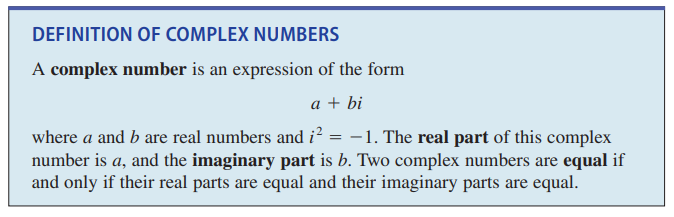
\includegraphics[width=1.1\textwidth]{algebra-pre-calculus/complex-numbers/complex_numbers_def.png}
\end{align*}

In the complex number the reason why $b$ is being called as the \textbf{imaginary part} is not because it's an imaginary number(when squared produce negative outcome). It's because it's being multiplied by the imaginary number $i$, so it's kind of the "part" of it. The real part is the part that is \textbf{not} being multiplied by $i$. \\

Note that both the real and the imaginary part are real numbers. 

A number such as $6i$, which has real part 0, is called a \textbf{pure imaginary number}. A
real number such as $-7$ can be thought of as a complex number with imaginary part 0.
In the complex number system every quadratic equation has solutions. The numbers
$2i$ and $-2i$ are solutions of $x^2-4$ because

\begin{align*}
    (2i)^2&=4i^2=-4 \\
    (-2i)^2&=4i^2=-4
\end{align*}

We study complex numbers because they complete, in a useful and elegant
fashion, our study of the solutions of equations. In fact, imaginary numbers are useful not
only in algebra and mathematics, but in the other sciences as well. To give just one example, in electrical theory the reactance of a circuit is a quantity whose measure is an
imaginary number. \\

\subsection{Arithmetic Operations on Complex Numbers}

Complex numbers are added, subtracted, multiplied, and divided just as we would any
number of the form $a+b\sqrt{c}$. The only difference that we need to keep in mind is that $i^2=-1$. Thus the following calculations are valid.

\begin{align*}
    (a+bi)(c+di)&= ac+adi+bci+bdi^2 \\
    &=ac+(ad+bc)i-bd \\
    &= (ac-bd)+(ad+bc)i
\end{align*}

\begin{align*}
    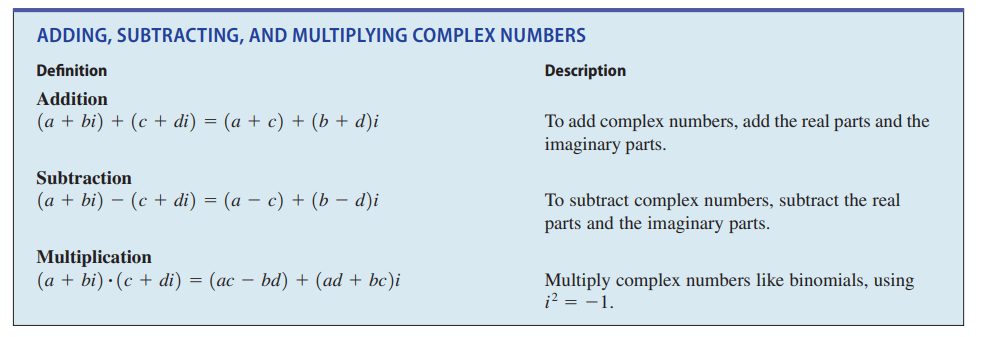
\includegraphics[width=1.1\textwidth]{algebra-pre-calculus/complex-numbers/arithmetic_operations_complex_numbers.png}
\end{align*}

\subsection{Examples of Adding and subtracting complex numbers}
\textbf{(a)} $(3+5i)+(4-2i)=(3+4)+(5-2)i=7+3i$ % Section 15 - Complex Numbers
% Chapter 1 end - Algebra

% Chapter 2 - Data Science 
\chapter{Data Science}

\chapter{Neural Networks with python}
\section{Introduction}

The concept of weights and biases can be thought of as “knobs” that we can tune to fit our model
to data. In a neural network, we often have thousands or even millions of these parameters tuned
by the optimizer during training. Some may ask, “why not just have biases or just weights?”
Biases and weights are both tunable parameters, and both will impact the neurons’ outputs, but
they do so in different ways. Since weights are multiplied, they will only change the magnitude or
even completely flip the sign from positive to negative, or vice versa. Output = weight·input+bias
is not unlike the equation for a line y = mx+b. We can visualize this with:
Weights set the standards for the neuron's signal strength. This value will determine the influence input data has on the output product. Biases give extra characteristics with a value of 1 that the neural network did not previously have.

To understand the effect in regards the steepness of the function with weights and biases watch this: \url{: https://nnfs.io/bru}

As a very general overview, the step function meant to mimic a neuron in the brain, either “firing”
or not — like an on-off switch. In programming, an on-off switch as a function would be called a
step function because it looks like a step if we graph it.

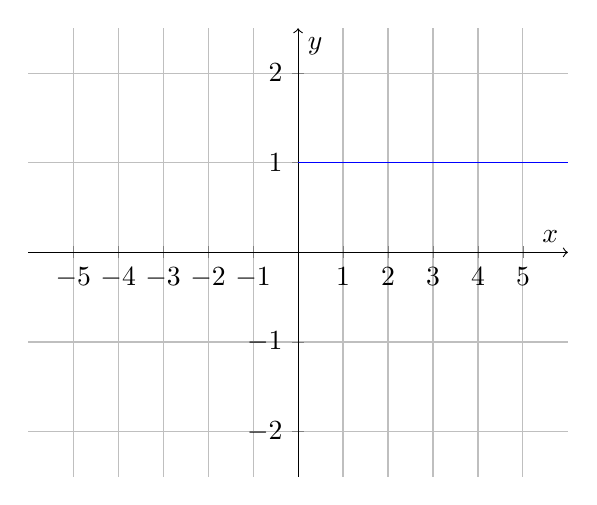
\begin{tikzpicture}
    \begin{axis}[
        xlabel={$x$},
        ylabel={$y$},
        axis lines=middle,
        axis line style={->},
        xmin=-6,
        ymin=-2.5,
        xmax=6,
        ymax=2.5,
        xtick={-5,-4,-3,-2,-1,0,1,2,3,4,5},
        ytick={-2,-1,0,1,2},
        legend style={at={(0.95,0.95)},anchor=north east},
        grid=both
      ]
        \addplot[domain=0:10, samples=100, color=blue]{1};
    \end{axis}
\end{tikzpicture} \\

\begin{equation*}
    |y| = \begin{cases}
        \;1  & x>0 \\
        \;0 & x \leq 0
    \end{cases}
\end{equation*}


discussing the concept of a "step function" in the context of neural networks and how it's used to model the behavior of neurons. Let me break it down for you:

\begin{itemize}
    \item In the brain, neurons are the basic functional units. They receive input signals from other neurons and, if the sum of those inputs reaches a certain threshold, the neuron "fires" or activates, transmitting a signal to other neurons. This activation is like turning on a switch, and it's a fundamental concept in neural activity.
    \item Step  When designing artificial neural networks (like those used in machine learning and deep learning), we often want to model the behavior of biological neurons. In this context, the "step function" is a simple mathematical function used to mimic the behavior of neurons.
    \item Think of the step function as an "on-off switch." If the input to the step function exceeds a certain threshold, the function's output is "on" (1), and if the input is below the threshold, the output is "off" (0). This behavior closely resembles the way biological neurons work, as they either fire or do not fire.
    \item The term "step" in the step function comes from the shape of its graph. When you plot this function on a graph, it looks like a step, where the output suddenly changes from 0 to 1 (or vice versa) at a specific threshold value.
\end{itemize}

In the previous function, x represents the input to the neuron, and \textbf{threshold}(whether the input is smaller or bigger than 0) is the value at which the neuron "fires." If x is less than the threshold, the output is 0 (off), and if x is greater than or equal to the threshold, the output is 1 (on).
In other words
For a step function, if the neuron’s output value, which is calculated by $sum(inputs\cdot weights)$
$+ bias$, is greater than 0, the neuron fires (so it would output a 1). Otherwise, it does not fire
and would pass along a 0. The formula for a single neuron might look something like:

 % Section 1 - Introduction

% Chapter 3 - Introduction to AI and ML %
\chapter{AI and Machine Learning}
\section{Supervised and Unsupervised Learning}

\subsection{Supervised Learning1}
Supervised learning is a type of machine learning algorithm that uses a known dataset (called the training dataset) to make predictions. The training dataset includes input data and output data. The key of supervised learning is that you give your learning algorithm examples to learn from that include the "right answers", in other words the correct label \textbf{y} for the input \textbf{x}.
It learns by seeing correct pairs of inputs and outputs.  The goal is that eventually the algorithm will only be provided with the input-value(x) and it has to predict the output-value/label(y). 
Examples: \\ \\ \\

\begin{align*}
    \scalebox{1.3}{
\begin{tabular}{|c|c|c|}
    \hline
    Input(x) & Output(y) & Application \\
    \hline
    email & spam?(0/1) & spam filtering \\
    \hline
    audio & text transcript & speech recognition \\
    \hline
    English & Spanish & machine translation \\
    \hline
    ad,user,info & click?(0/1) & online advertising \\
    \hline
    image, radar info & position of other cars & self-driving car \\
    \hline
    image of a phone & defect?(0/1) & visual inspection \\
    \hline
\end{tabular}}
\end{align*}

In all of these applications you first train your model on data where you know the correct output. Then you use that model to make predictions on new data. \\

\subsubsection*{Regression: Housing Price Prediction}
Regression is a type of supervised learning algorithm that tries to predict a continuous output variable. In other words, it is used to predict a number. For example, predicting the price of a house in dollars is a regression problem whereas predicting whether a tumor is malignant or benign is a classification problem. \\
In other words, Regression is a type of algorithm that tries to predict a continuous output variable. 

\subsubsection*{Classification: Breast Cancer Prediction}
Say that you are trying to create a model that predicts whether or not a tumor is malignant or benign. In classification problems, the output variable is a category (such as "malignant" or "benign"). What we are trying to do is map input variables to discrete categories, we are classifying the input values into categories and trying to predict from the two possible output. Here we have a number of possible categories or outputs that our algorithm can predict. Whereas with regression we are trying to predict a continuous number. 
To summarise, Classification is a type of algorithm that tries to predict a discrete category, that doesn't necessarily have to be a number. Also in classification we are predicting a small set of possible outputs, so we are given our "options" in regards of what can our output be.
By extension obviously, we can have two or more inputs, in this case we can think of inputs as a "context" dataset that is provided to us, such as the tumor size, or the patient's age, sex, etc... The more context we provide the more accurate our prediction will be.
What we often do is represent our data-set in a function for example and our algorithm would try to identify some form of pattern in the data-set.

\subsection{Summary of Supervised Learning}
In summary supervised learning is when we are given a data-set and we are told what our correct output should be. We are given the "right answers" and we are trying to learn from that data-set to be able to predict the correct output for new data without the need of the input.
We have looked at two categories of supervised learning, regression and classification. In regression we are trying to predict a continuous number, and in classification we are trying to predict a discrete category.


\subsection{Unsupervised Learning}

Previously, in our classification problem what we have looked at is a supervised learning problem. We have a data-set and we are given the correct output(y) for each example. In unsupervised learning we are given a data-set but we are \textbf{not} given any labels or output value(y). Say you were given with the tumor size and the patient's age and any other context, however you don't know whether the tumor is malignant or benign. You are not given any labels or output value. 
Our job here is not to predict whether the tumor is malignant or benign, but rather to find some structure in the data-set. In other words find something interesting in the unlabeled data-set. 
The reason why it is called unsupervised is because we are not supervising the algorithm, we are not telling it what the correct answer is, we are just giving it the data and asking it to find some structure in the data.
So it might identify that the data can be divided into number of sections, or it might find some form of patterns between the patient's age and their tumor size, or any other contextual prediction.
Essentially it tries to place the data into different clusters, clustering is a type of unsupervised learning, where we are trying to find some structure in the data. For example clustering is used in google news. 
What google news does is every day it goes through all the news articles that are published and it tries to group them into different clusters, so that it can show you the different clusters of news articles and you can choose which cluster you are interested in.

Another type of unsupervised learning is anomaly detection where we are trying to find some abnormal behavior in the data. For example, if we have a data-set of credit card transactions and we are trying to find some unusual behavior in the data-set, such as unusual credit card transactions.
Another example is in manufacturing, where we are trying to find some unusual behavior in the manufacturing process, such as unusual defects in the product.
We also have dimensionality reduction where we are trying to take a data-set with a large number of features and reduce the number of features to a smaller number. For example, if we have a data-set with a large number of features, we might want to reduce the number of features to a smaller number so that we can visualize the data more easily.

\subsection{Linear Regression: House sizes and prices}
In this example let's imagine that we are given with a data-set about house prices and their sizes. We are given the size of the house in square feet and the price of the house in dollars. We are given a number of examples of houses and their prices. We are trying to predict the price of a new house given its size.
This is a perfect example of a linear regression model where we would first train our model on the data-set and showing the "right answers" and then we can use that model to predict the price of a new house given its size.

A data-set that is used to train a model is called a training set. The sizes of the house can be represented with x as for example if we  have a house that is 1000 square feet, we can represent that with x = 1000. The price of the house can be represented with y, so if the price of the house is 200,000 dollars, we can represent that with y = 200,000. 

We call x as the "input" variable or feature, and refer to y as the "output" variable or target. 

We can represent as a single training example by $$(x,y)$$ where x is the input and y is the output.
Our $i$th training example where I would represent a specific row from the training set would look like this: $(x^{(i)},y^{(i)})$.

Note that this doesn't mean that we are taking x and y to the power of i, but rather that we are taking the i'th training example from the training set.

So for example one example would look like this $$ (x^{(1)}, y^{(1)})=(2104,400) $$

Also as mentioned $$x^{(2)}\neq x^2$$

\subsection{Process of a Supervised training}
Supervised learning algorithm will input a dataset and then what exactly does it do and what does it output? 
Recall that a training set in supervised learning includes both the input features, such as the size of the house and also the output targets, such as the price of the house. The output targets are the right answers to the model we'll learn from.
To train the model, you feed the training set, both the input features and the output targets to your learning algorithm.  % Section 1 - Supervised and Unsupervised Learning
\end{document}

